\documentclass[aspectratio=169]{beamer}
\usepackage{fontspec}
\setmainfont{Arial}

% --- PACKAGES ---
\usepackage[english]{babel}
\usepackage{graphicx}
\usepackage{booktabs}
\usepackage{tcolorbox}
\usepackage{fontspec}
\usepackage{caption}
\captionsetup[figure]{labelformat=empty}
\usepackage{xcolor}
\usepackage{tikz} % Needed for \tikz \path commands
\usepackage{csquotes}
\usepackage{listings}

\usepackage[backend=biber, style=apa, doi=true]{biblatex}
\renewcommand*{\bibfont}{\normalfont\scriptsize}
\addbibresource{bib/14281892.bib}
\addbibresource{bib/berners.bib}
\addbibresource{bib/turning.bib}
\addbibresource{bib/fair.bib}
\addbibresource{bib/platforms.bib}
\addbibresource{bib/guide.bib}
\addbibresource{bib/5727048.bib}




% 1. COLOR DEFINITIONS (KIT & HMC)
\definecolor{KITBlue}{RGB}{0, 98, 148}
\definecolor{HMCBlue}{RGB}{0, 40, 100}
\definecolor{HMCAccent}{RGB}{20, 200, 255}
\definecolor{HMCMint}{RGB}{5, 229, 186}
\definecolor{HMCClaim}{RGB}{0, 128, 64}
\definecolor{LightGray}{RGB}{242, 242, 242}
\definecolor{VeryLightGray}{RGB}{252, 252, 252}


% 2. THEME APPLICATION (Minimalist)
\usefonttheme{professionalfonts}
\useinnertheme{default}
\useoutertheme{miniframes} % Minimalist header
% \setbeamertemplate{navigation symbols}{} % No navigation symbols

% Custom Footline Definition to insert the logo
\setbeamertemplate{footline}{
  \leavevmode
  \hbox{
    % Right box: Logo and Frame Number
    \begin{beamercolorbox}[wd=\paperwidth,ht=2.25ex,dp=1ex,right]{date in head/foot}
        \raisebox{-0.8ex}{
\includegraphics[width=6ex]{figs/kit_logo}}
      \raisebox{-0.4ex}{
\includegraphics[width=10ex]{figs/hmc_logo}}|
      \usebeamerfont{date in head/foot}\insertframenumber\hspace*{8ex}
    \end{beamercolorbox}}
    \vskip1ex
}

% 3. BEAMER COLOR SCHEMES
\setbeamercolor{palette primary}{fg=white, bg=HMCBlue}
\setbeamercolor{section in head/foot}{fg=white, bg=HMCBlue}
\setbeamercolor{palette secondary}{fg=white, bg=HMCAccent}
\setbeamercolor{structure}{fg=HMCAccent}
\setbeamercolor{local structure}{fg=HMCAccent}
\setbeamercolor{title}{bg=HMCBlue, fg=LightGray}
\setbeamercolor{frametitle}{fg=HMCBlue, bg=white}
\setbeamercolor{block title}{fg=HMCClaim, bg=LightGray}
\setbeamercolor{block body}{fg=HMCBlue, bg=VeryLightGray}
\setbeamercolor{author in head/foot}{bg=white, fg=HMCBlue}
\setbeamercolor{title in head/foot}{bg=white, fg=HMCBlue}
\setbeamercolor{date in head/foot}{bg=white, fg=HMCBlue}

% 4. FONT CONFIGURATION
% (Requires Noto Sans to be installed on your system)
%% \setmainfont{Noto Sans} 
%% \setsansfont{Noto Sans}
\lstdefinelanguage{XML}{
    basicstyle=\ttfamily\tiny,
    showstringspaces=false,
    breaklines=true,
    frame=lines,
    literate={>}{{{\color{HMCAccent}>}}}1
             {<}{{{\color{HMCAccent}<}}}1
}
\lstdefinelanguage{yaml}{
    basicstyle=\ttfamily\tiny,
    showstringspaces=false,
    breaklines=true,
    frame=lines,
    literate=
   % {  }{
   %   \makebox[0.5em][l]{\colorbox{HMCMint}{\phantom{p}}}
   %   \makebox[0.5em][l]{\colorbox{HMCMint}{\phantom{p}}}
   % }{2}
             {,}{{{\color{HMCAccent},}}}1
             {:}{{{\color{HMCAccent}:}}}1
             {[}{{{\color{HMCAccent}{[}}}}1
             {]}{{{\color{HMCAccent}{]}}}}1
             {\{}{{{\color{HMCAccent}{\{}}}}1
             {\}}{{{\color{HMCAccent}{\}}}}}1
}
\lstdefinelanguage{json}{
    basicstyle=\ttfamily\tiny,
    showstringspaces=false,
    breaklines=true,
    frame=lines,
    literate={"}{{{\texttt{\char34}}}}1
             {,}{{{\color{HMCAccent},}}}1
             {:}{{{\color{HMCAccent}:}}}1
             {[}{{{\color{HMCAccent}{[}}}}1
             {]}{{{\color{HMCAccent}{]}}}}1
             {\{}{{{\color{HMCAccent}{\{}}}}1
             {\}}{{{\color{HMCAccent}{\}}}}}1
}
\lstdefinelanguage{CSV}{
    basicstyle=\ttfamily\tiny,
    showstringspaces=false,
    breaklines=true,
    frame=lines,
    literate={,}{{{\color{HMCAccent},}}}1
    {;}{{{\color{HMCAccent};}}}1, 
}

% 5. Define the switch \ifenablepauses
\newif\ifenablepauses
% Set the default state
\enablepausestrue           % (for animated presentation)
\enablepausesfalse          % (for static presentation)


% --- METADATA & TITLE GRAPHICS ---
\title{Metadata for Scientific Data Integrity}
\subtitle{for Energy}
\author{IG Training - HMC, Anis Koubaa, Nan Liu}%, Mirl Törsch}
\institute{Karlsruhe Institute of Technology (KIT) \\
\vspace{.4em}
    
\includegraphics[height=0.32cm]{figs/kit_logo.png}
    \vspace{.4em}}

\date{24. March 2026}

% Add logos to the title page. 
% Make sure 'kit_logo.png' and 'hmc_logo.png' are in the same folder.
\titlegraphic{
    \vspace{1.6em}
    \includegraphics[height=0.64cm]{figs/hmc_Logo.png}
}


% ===================================================================
% DOCUMENT BEGINS
% ===================================================================

\AtBeginDocument{
    \ifenablepauses % Do nothing, \pause retains its normal behavior
    \else % If pauses are disabled, redefine \pause to be an empty command (equivalent to \relax)
      \let\pause\relax
    \fi}
    

\begin{document}

% --- TITLE PAGE ---
%\begin{frame}[plain]
%   % Use tikz to draw the image at the background layer (lower)
%   \tikz[overlay, remember picture] \path (current page.south west) node[anchor=south west] {
%       
\includegraphics[width=\paperwidth]{figs/HMC-Training_Integrity_20251121-20_Indico.jpg}
%   };
%
%\end{frame}

\begin{frame}[plain]

    \titlepage
    
\end{frame}

% --- AGENDA ---
{
    \setbeamertemplate{background canvas}{
        
\includegraphics[width=\paperwidth,height=\paperheight]{figs/background_white.png}
    }
    \begin{frame}[plain]{Our Target: Publish a distribution of some datasets, on two different platforms}
        \begin{block}{How we will Work}
            \begin{enumerate}
                \item \textbf We explore the core concepts and the "why"
                \item \textbf We look at practical cases:
                    \begin{itemize}
                        \item Measured active power photovoltaic on the top roof of IAI, after aggregation
                        \item Data gathered from an MQTT Broker
                        \item The content of this training material for future reference
                    \end{itemize}
        \end{enumerate}
        \end{block}
    \end{frame}
}

% ===================================================================
% PART 1: From Data Integrity to FAIR Principles
% ===================================================================

\section{Intro: Integrity to FAIR}
{
    \setbeamertemplate{background canvas}{
        
\includegraphics[width=\paperwidth,height=\paperheight]{figs/background_white.png}
    }
    
    \begin{frame}[plain]{Part 1: From Data Integrity to FAIR}{09:15 - 09:45}
        \begin{block}{Goal}
            To connect the foundational, ethical duty of \textbf{Data Integrity} to the modern, practical framework of the \textbf{FAIR Principles}.
        \end{block}
        \begin{center}
            
\includegraphics[width=0.56\textwidth]{figs/fig_d1p1/d1p1_01-fairintegrity.png}
        \end{center}
    \end{frame}
}

\begin{frame}{Learning Objectives}
    \begin{itemize}
        \item \textbf{Define} the core concepts of \textbf{Data Integrity} (accuracy, completeness, and consistency) and the four pillars of the \textbf{FAIR} acronym.
        \item \textbf{List} three Guidelines from the DFG code of conduct concerning Data Integrity.
    \end{itemize}
\end{frame}

\begin{frame}{Theory: What is Data Integrity?}{Define}
    \begin{columns}
        \column{.36\textwidth}
        \begin{center}
            
\includegraphics[width=\textwidth]{figs/fig_d1p1/d1p1_02-integrity.png}
        \end{center}
        \column{.64\textwidth}
        \textbf{Data Integrity} is the maintenance and assurance of the \textbf{accuracy}, \textbf{completeness}, and \textbf{consistency} of data over its entire life-cycle.
        \pause
        \begin{itemize}
            \item \textbf{Accuracy:} Data reflects the real-world event. It is correct and precise.
            \pause
            \item \textbf{Completeness:} No critical data is missing. The dataset is whole.
            \pause
            \item \textbf{Consistency:} Data is uniform. The same value is represented the same way everywhere (e.g., `KIT` vs. `Karlsruhe Institute of Technology`).
        \end{itemize}
    \end{columns}
\end{frame}

\begin{frame}{Theory: What are the FAIR Principles?}{Define}
    The FAIR Principles are a set of guiding principles to make research data more valuable and reusable.
    
    \begin{itemize}
        \item \textbf{F}indable: Data (and metadata) must be easy to find by both humans and machines. (e.g., Persistent Identifiers - PIDs).
        \pause
        \item \textbf{A}ccessible: Once found, the (meta)data must be retrievable via a standard protocol. (e.g., HTTP, FTP).
        \pause
        \item \textbf{I}nteroperable: Data must be able to be combined with other datasets, using formal, shared languages and vocabularies.
        \pause
        \item \textbf{R}eusable: Data must be richly described with metadata and have a clear license so it can be replicated or combined.
    \end{itemize}
    More details? \href{https://www.go-fair.org/wp-content/uploads/2022/01/FAIRPrinciples_overview.pdf}{GOFAIR}
\end{frame}

\begin{frame}{Concept: DFG Code of Conduct}{List}
    Data Integrity is a core component of the DFG "Guidelines for Safeguarding Good Research Practice." 
    \cite{deutsche_forschungsgemeinschaft_2025_14281892}
    
    
    \begin{block}{Key Guidelines on Integrity}
        \begin{itemize}
            \item \textbf{Guideline 7 (Safeguarding and Storing):} Researchers safeguard their research data and document the steps taken.
            \pause
            \item \textbf{Guideline 12 (Documentation):} Documentation and re- search results must not be manipulated; they are protected as effectively as possible against manipulation.
            \pause
            \item \textbf{Guideline 17 (Archiving):} Primary data must be securely archived for a minimum of ten years.
        \end{itemize}
    \end{block}
\end{frame}

\begin{frame}{Interactive: Defining Our Terms}{Practice}
    \begin{block}{Group Discussion (8 min)}
        Let's put this together.
        \begin{itemize}
            \item In your own words, what is the biggest threat to \textbf{Data Integrity} in your specific research field?
            \pause
            \item Which of the four \textbf{FAIR} principles do you find the most challenging to implement?
            \pause
            \item How do \textbf{Guideline 12 (\href{https://wissenschaftliche-integritaet.de/en/code-of-conduct/documentation/}{Documentation})} and the 'R' (Reusable) principle relate?
        \end{itemize}
    \end{block}
    \href{https://miro.com/app/board/uXjVJpI_9Kc=/?moveToWidget=3458764648827295133&cot=14}{$\therefore$ Let's miro (How do GRP12 and ’R’ relate)?}
\end{frame}

\begin{frame}{Learning Objectives}
    \begin{itemize}
        \item \textbf{Explain} the \textbf{causal relationship} between maintaining high \textbf{Data Integrity} during collection and achieving the \textbf{Reusability} ('R') principle.
        \item \textbf{Explain} how adhering to the FAIR-Principles is crucial to reach accordance with the DFG guidelines.
    \end{itemize}
\end{frame}

\begin{frame}{Theory: The Integrity-Reusability Chain}{Explain}
    \begin{center}
        \textbf{High Data Integrity} $\rightarrow$ \textbf{Trust} $\rightarrow$ \textbf{Reusability}
    \end{center}
    \vfill
    \begin{itemize}
        \item \textbf{Reusability ('R')} is the ultimate goal of FAIR. It means someone else (or you, in 5 years) can understand, trust, and reuse your data.
        \pause
        \item This is \textbf{impossible} without Data Integrity.
        \pause
        \item If your data is \textbf{inaccurate}, reusing it gives wrong results.
        \item If your data is \textbf{incomplete}, reusing it is impossible.
        \item If your data is \textbf{inconsistent}, reusing it requires massive, error-prone cleaning.
    \end{itemize}
\end{frame}

\begin{frame}{Concept: The Broken Chain}{Explain}
    \begin{block}{Example of Low Integrity}
        A research group publishes a dataset on material strength.
        \begin{itemize}
            \item Column `temp`: Contains values `25C`, `298K`, and `25`.
            \item Column `pressure`: Contains values `1 atm`, `101.3 kPa`, and `1.013`.
        \end{itemize}
        This data is \textbf{inconsistent}.
    \end{block}
    \pause
    \begin{block}{Impact on Reusability}
        A second researcher tries to reuse this data for a meta-analysis. They cannot trust the values. They cannot automate a script. The data is \textbf{not reusable}. The 'R' principle fails.
    \end{block}
\end{frame}

\begin{frame}{Theory: FAIR as a Tool for DFG Concordance}{Explain}
    The DFG Guidelines tell you \textbf{what} to do (e.g., "Archive data", "Document results").
    \pause
    The FAIR Principles tell you \textbf{how} to do it effectively for the modern, digital age.
    
    \begin{itemize}
        \item \textbf{DFG Guideline 7 (Cross-phase quality assurance)} $\rightarrow$ Is achieved by implementing 'R' (Reusable), which requires rich metadata.
        \pause
        \item \textbf{DFG Guideline 12 (Documentation)} $\rightarrow$ Is achieved by implementing domain specific guidelines for assessment and review, along with strong provenance, enabling Interoperability (I).
        \pause
        \item \textbf{DFG Guideline 13 (Providing public access to research results)} $\rightarrow$ Is achieved by implementing 'F' (Findable) with a PID and 'A' (Accessible) in a repository.
    \end{itemize}
    \href{https://miro.com/app/board/uXjVJpI_9Kc=/?moveToWidget=3458764648818228865&cot=14}{$\therefore$ Let's miro (Categories of Metadata for DFG Compliance)?}    
\end{frame}

\begin{frame}{Interactive: The Broken Chain}{Practice}
    \begin{block}{Think-Pair-Share (10 min)}
        \textbf{Scenario:} A researcher leaves KIT. Their raw data is on a USB drive in their desk. The only "documentation" is their published paper.
        \pause
        \textbf{Discuss:}
        \begin{itemize}
            \item Which \textbf{Data Integrity} principles are broken?
            \item Which \textbf{FAIR} principles are broken?
            \item Which \textbf{DFG Guidelines} are broken?
        \end{itemize}
        \pause
        \textbf{Goal:} \textbf{Explain} how these three concepts are deeply linked.
    \end{block}
\end{frame}

\begin{frame}{Learning Objectives}
    \begin{itemize}
        \item \textbf{Apply} data validation and cleaning techniques (e.g., scripting checks, normalisation) to a raw dataset.
        \item \textbf{Write} a checklist to help Researchers assess their own concordance with the guidelines.
    \end{itemize}
\end{frame}

\begin{frame}{Theory: What is Data Validation?}{Apply}
    Data Validation is the set of processes used to ensure data has high \textbf{integrity} (accuracy, completeness, consistency).
    \pause
    \begin{columns}
        \column{.64\textwidth}
        \textbf{Techniques:}
        \begin{itemize}
            \item \textbf{Range Checks:} Is a pH value 15? (Invalid)
            \item \textbf{Format Checks:} Is a date `YYYY-MM-DD`?
            \item \textbf{Normalisation:} Converting all units (C, K) to one standard (K).
            \item \textbf{Schema Validation:} Does the data conform to the rules we set?
        \end{itemize}
        
        \column{.36\textwidth}
        \begin{center}
            
\includegraphics[width=.8\textwidth]{figs/fig_d1p1/d1p1_03-validation_check.png}
            \captionof{figure}{Validation as a Quality Control Checkpoint}
        \end{center}
    \end{columns}
\end{frame}

\begin{frame}[fragile]{Concept: Validation in Practice (Pseudo-Code)}{Apply}
    
    You don't have to check data manually! Use scripts.
    
    \begin{block}{Simple Python Check (Pseudo-code)}
\begin{verbatim}
data = read_csv("my_experiment.csv")
for row in data:
    # Check for completeness (e.g., no missing IDs)
    if row['sample_id'] is None: print("Error: Missing sample_id!")
    # Check for consistency (e.g., standardising units to Kelvin)
    if row['unit'] == "C": row['temp_K'] = convert_to_kelvin(row['temp'])
    # Check for range (e.g., no impossible values below absolute zero)
    if row['temp_K'] < 0: print("Error: Impossible temperature!")
save_csv("my_clean_data.csv", data)
\end{verbatim}
    \end{block}
\end{frame}

\begin{frame}{Interactive: The Concordance Checklist}{Practice}
    \begin{block}{Activity: Write a Checklist (15 min)}
        You are onboarding a new PhD student.
        \pause
        \textbf{Task:} Draft a 5-point "Data Integrity Checklist" to help them assess their own concordance with DFG guidelines.
        \pause
        \begin{itemize}
            \item \emph{Example 1: (Completeness)} "Does every dataset have a `README` file?"
            \item \emph{Example 2: (Consistency)} "Is there a script to check that all units are standardised?"
            \item \emph{Example 3: (Accuracy)} "Has a colleague double-checked the manual data entry?"
        \end{itemize}
        \pause
        \textbf{Goal:} \textbf{Write} this checklist. We will share them.
    \end{block}
    \href{https://miro.com/app/board/uXjVJpI_9Kc=/?moveToWidget=3458764649162553531&cot=14}{$\therefore$ Let's miro (Onboarding)}
\end{frame}

\begin{frame}{Learning Objectives}
    \begin{itemize}
        \item \textbf{Differentiate} between the requirements for data \textbf{Authenticity} (Integrity) and data \textbf{Accessibility} (FAIR).
        \item \textbf{Identify} criteria of publication platforms.
    \end{itemize}
\end{frame}

\begin{frame}{Theory: Authenticity vs. Accessibility}{Differentiate}
    These two concepts are often confused, but are very different.
    
    \begin{columns}
        \column{.5\textwidth}
        \begin{block}{Authenticity (Data Integrity)}
            \textbf{Question:} Is this the \emph{real, unaltered} data?
            \pause
            \textbf{Method:}
            \begin{itemize}
                \item Checksums (e.g., MD5, SHA256)
                \item Digital Signatures
                \item Audit Trails
                \item Version Control History
            \end{itemize}
            \textbf{Metaphor:} A sealed, tamper-proof envelope.
        \end{block}
        
        \column{.5\textwidth}
        \begin{block}{Accessibility (FAIR Principle 'A')}
            \textbf{Question:} Can I \emph{get} to the data?
            \pause
            \textbf{Method:}
            \begin{itemize}
                \item A Persistent Identifier (PID)
                \item A standard protocol (e.g., HTTP)
                \item An open, public URL
                \item Clear authentication (if not open)
            \end{itemize}
            \textbf{Metaphor:} A public mailbox with a clear address.
        \end{block}
    \end{columns}
\end{frame}

\begin{frame}{Concept: PIDs as the Bridge}{Differentiate}
    Persistent Identifiers (like a DOI) are the bridge between Authenticity and Accessibility.
    
    \begin{itemize}
        \item A PID (like a DOI from zenodo) makes the data \textbf{Accessible} ('A') by giving it a permanent,
        findable web address.
        \pause
        \item The repository \textit{behind} the DOI (zenodo) ensures \textbf{Authenticity} (Integrity) by storing the
        file and often providing a checksum (MD5/SHA) to prove it hasn't been altered since publication.
    \end{itemize}
    \pause
    \begin{block}{Key Idea}
        You can have Authenticity without Accessibility (e.g., a file on a secure, offline server).
        \pause
        You should \textit{never} have Accessibility without Authenticity (e.g., a public file that anyone can edit).
    \end{block}
\end{frame}

\begin{frame}{Theory: Criteria for Publication Platforms}{Identify}
    When choosing \textit{where} to publish, you must \textbf{identify} its criteria.
    \begin{itemize}
        \item \textbf{Findability-Degree:} This is key.
        \pause
        \item \textbf{Level 1 (Low):} Publishes data (e.g., a project website).
        \pause
        \item \textbf{Level 2 (Good):} Publishes data + assigns a PID (e.g., KITOpen).
        \pause
        \item \textbf{Level 3 (Excellent):} Publishes data + PID + rich, machine-readable, \emph{domain-specific} metadata (e.g., Open Energy Platform).
    \end{itemize}
    \pause
    \begin{block}{Other Criteria}
        \textbf{Check for:} PID minting (DOIs?), license support (CC-BY?), long-term preservation plan, costs, access control (embargoes?).
    \end{block}
\end{frame}

\begin{frame}{Interactive: Platform Criteria}{Practice}
    \begin{block}{Discussion (10 min)}
        \textbf{Task:} Let's \textbf{identify} criteria for publication platforms.
        \begin{itemize}
            \item What is the "findability-degree" of putting your data on a personal website?
            \pause
            \item What about on a GitHub repository?
            \pause
            \item What about on zenodo?
        \end{itemize}
        \pause
        \textbf{Question:} Why is a high "findability-degree" so important for both you (impact) and your field (progress)?
    \end{block}
    More? \cite{koubaa_energy_2025}
\end{frame}

\begin{frame}{Learning Objectives}
    \begin{itemize}
        \item \textbf{Appraise} a current data storage system against both the criteria for long-term \textbf{Data Security} (Integrity) and \textbf{machine accessibility} ('A' of FAIR).
        \item \textbf{Describe} the importance of the find-ability-degree in selecting where to publish.
    \end{itemize}
\end{frame}

\begin{frame}{Theory: Criteria for Storage vs. Access}{Appraise}
    We must evaluate storage on two axes: Safety (Integrity) and Openness (FAIR).
    
    \begin{columns}
        \column{.5\textwidth}
        \begin{block}{Data Security (Integrity)}
            \textbf{Question:} Is my data safe?
            \begin{itemize}
                \item \textbf{Durability:} Is it backed up?
                \item \textbf{Security:} Who has access?
                \item \textbf{Auditing:} Can I see who changed what? (Version history)
            \end{itemize}
            \begin{center}
                
\includegraphics[width=.24\textwidth]{figs/fig_d1p1/d1p1_04-fortress.png}
            \end{center}
            %\caption{A secure fortress.}
        \end{block}
        
        \column{.5\textwidth}
        \begin{block}{Machine Accessibility ('A')}
            \textbf{Question:} Can a machine get it?
            \begin{itemize}
                \item \textbf{Protocol:} Is it on `http` or `ftp`?
                \item \textbf{Identifier:} Does it have a PID/DOI?
                \item \textbf{Metadata Access:} Is metadata accessible, even if data is restricted?
            \end{itemize}
            \begin{center}
                
\includegraphics[width=.24\textwidth]{figs/fig_d1p1/d1p1_05-openess.png}
            \end{center}
            %\caption{A robot accessing a library.}
        \end{block}
    \end{columns}
\end{frame}

\begin{frame}{Concept: Evaluating Storage Options}{Appraise Storage Solutions}
    
    Let's appraise common storage systems against our ethical duties.
    \begin{center}
        \begin{tabular}{p{0.24\textwidth}|p{0.33\textwidth}|p{0.33\textwidth}}
            \toprule
            \textbf{Storage System} & \textbf{Data Security (Integrity)} & \textbf{Machine Access ('A')} \\
            \midrule
            
            % Use \pause immediately before the text to be revealed
            \pause
            Your Laptop HD & \textcolor{HMCBlue!40}{\textbf{Very Low}\newline (No backup, easily lost)} & \textcolor{HMCBlue!20}{\textbf{None}\newline (Offline)} \\
            \addlinespace
            
            % \pause is now used only at the start of the row to make the whole row appear.
            \pause
            Shared Drive & \textcolor{HMCBlue!80}{\textbf{Medium}\newline (Backed up, access control)} & \textcolor{HMCBlue!60}{\textbf{Low}\newline (Internal, not public)} \\
            \addlinespace
            
            \pause
            GitHub (Public) & \textcolor{HMCBlue}{\textbf{High}\newline (Versioned, backed up)} & \textcolor{HMCBlue!80}{\textbf{Medium}\newline (No PID, not a formal repo.)} \\
            \addlinespace
            
            \pause
            KITOpen (Repo.) & \textbf{Very High}\newline (Managed, backed up) & \textbf{Very High}\newline (Public, HTTP, PID) \\
            \bottomrule
        \end{tabular}
    \end{center}
\end{frame}

\begin{frame}{Interactive: Appraise Your Storage}{Practice}
    \begin{block}{Personal Evaluation (10 min)}
        \textbf{Task:} Think about the \emph{primary} place you store your "in-progress" research data right now.
        \begin{itemize}
            \item \textbf{Appraise} its \textbf{Data Security}. What is your biggest risk? (e.g., "My laptop gets stolen," "A colleague overwrites the file.")
            \pause
            \item \textbf{Appraise} its \textbf{Machine Accessibility}. Could an external collaborator (or a script) access it without you emailing it?
        \end{itemize}
        \pause
        \textbf{Share:} Let's hear some examples.
    \end{block}
\end{frame}

\begin{frame}{Learning Objectives}
    \begin{itemize}
        \item \textbf{Develop} a comprehensive, integrity-focused \textbf{Metadata Standard} that, when implemented, ensures the data meets all FAIR principles.
        \item \textbf{Distinguish} different types of interoperability (The 5 Stars).
    \end{itemize}
\end{frame}

\begin{frame}{Theory: What is a Metadata Standard?}{Develop}

    A Metadata Standard is not just a list of fields. It's a complete \textbf{"instruction manual"} for your data, essential for maintaining data integrity (\href{https://github.com/OpenEnergyPlatform/oemetadata}{an example?}).

    It must define:
    \begin{enumerate}
        \pause
        \item \textbf{Schema:} What fields are required? (e.g., \texttt{Creator}, \texttt{Date}, \texttt{Sample\_ID}).
        \pause
        \item \textbf{Vocabularies:} What are the allowed \textit{values} for a field? (e.g., For \texttt{Unit}, you must use \texttt{K}, \texttt{m}, or \texttt{kg}. No \texttt{Celsius} or \texttt{grams}.)
        \pause
        \item \textbf{Format:} How is it written? (e.g., "All metadata will be stored as a \texttt{metadata.json} file alongside the data.")
    \end{enumerate}
    \pause
    \begin{block}{Key Idea}
        An "integrity-focused" standard \textbf{requires} fields that ensure accuracy (e.g., \texttt{Instrument\_Calibration\_Date}) and consistency (e.g., \texttt{Unit\_Standard}).
    \end{block}
\end{frame}

\begin{frame}{Concept: The 5 Stars of Interoperability}{Distinguish}
    \begin{columns}
        
    \column{.36\textwidth}
    \begin{center}
        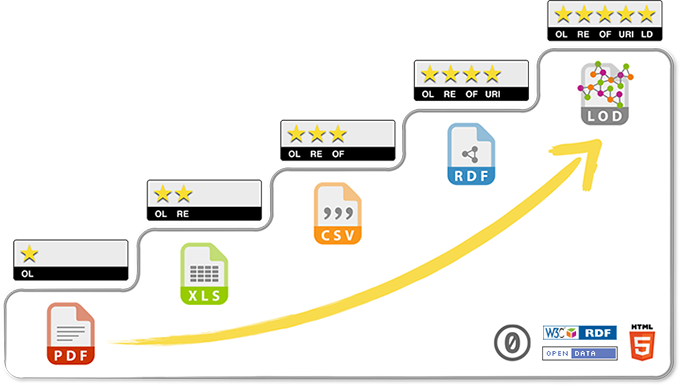
\includegraphics[width=\textwidth]{figs/fig_d1p1/5-star-steps.png} \cite{BernersLee5StarData}
    \end{center}
    \column{.64\textwidth}
    \begin{itemize}
        \item $\star$ -- Data is on the web (e.g., a PDF)
        \item $\star\star$ -- Machine-readable (e.g., an Excel file)
        \item $\star\star\star$ -- Non-proprietary format (e.g., a CSV file)
        \item $\star\star\star\star$ -- Uses URIs/PIDs as identifiers
        \item $\star\star\star\star\star$ -- \textbf{Links} to other data (Linked Open Data)
    \end{itemize}
    \pause
    This is the \href{https://5stardata.info/en/}{$\therefore$ ladder} we are trying to climb!
    \end{columns}
\end{frame}

\begin{frame}{Interactive: Brainstorm Your Standard}{Practice}
    \begin{block}{Workshop (8 min)}
        \textbf{Task:} Let's \textbf{develop} a \textit{minimal} metadata standard for a simple experiment.
        \pause
        \textbf{Scenario:} Measuring the temperature of 10 water samples.
        \pause
        \textbf{Brainstorm:} What fields are \textit{essential} for...
        \begin{itemize}
            % Fix: Escaping underscores with \_ within the \texttt{} environment
            \item \textbf{Integrity:} (e.g., \texttt{operator\_{name}}, \texttt{calibration\_{date}})
            \item \textbf{FAIRness:} (e.g., \texttt{sample\_{id}}, \texttt{unit}, \texttt{location\_{geocoordinates}})
        \end{itemize}
        \pause
        \textbf{Goal:} \textbf{Distinguish} between fields for simple documentation and fields for 5-star interoperability.
    \end{block}
    \href{https://miro.com/app/board/uXjVJpI_9Kc=/?moveToWidget=3458764649160876023&cot=14}{$\therefore$ Let's miro (temperature of 10 water samples)}
\end{frame}

\begin{frame}{Summary}
    \begin{itemize}
        \item \textbf{Data Integrity} (Accurate, Complete, Consistent) is the foundation.
        \item \textbf{FAIR Principles} are the practical framework for modern data.
        \item \textbf{DFG Guidelines} are the "law" that requires both.
        \item We apply integrity by \textbf{validation} and \textbf{appraising} our tools.
        \item We plan for FAIR by developing \textbf{Metadata Standards}.
        \item RDA Guidelines for publishing structured metadata on the web \cite{wu_2021_5727048} can be considered.
    \end{itemize}
    \vfill
    \begin{center}
        \textbf{End of Part 1}
    \end{center}
\end{frame}

\begin{frame}{Bibliography}
    \printbibliography
\end{frame}

% ===================================================================
% PART 2: Implementing The FAIR-Principles - Planning Phase
% ===================================================================

\section{Planning: The DMP}
{
    \setbeamertemplate{background canvas}{
        
\includegraphics[width=\paperwidth,height=\paperheight]{figs/background_white.png}
    }
    \begin{frame}[plain]{Day 1 - Part 2: The Planning Phase}{10:50 - 11:35}
        \begin{block}{Module 2 Goal}
            To master the \textbf{Data Management Plan (DMP)} as our primary tool for \textit{planning} a FAIR publication, using the \textbf{RDMO} tool.
        \end{block}
        \begin{center}
            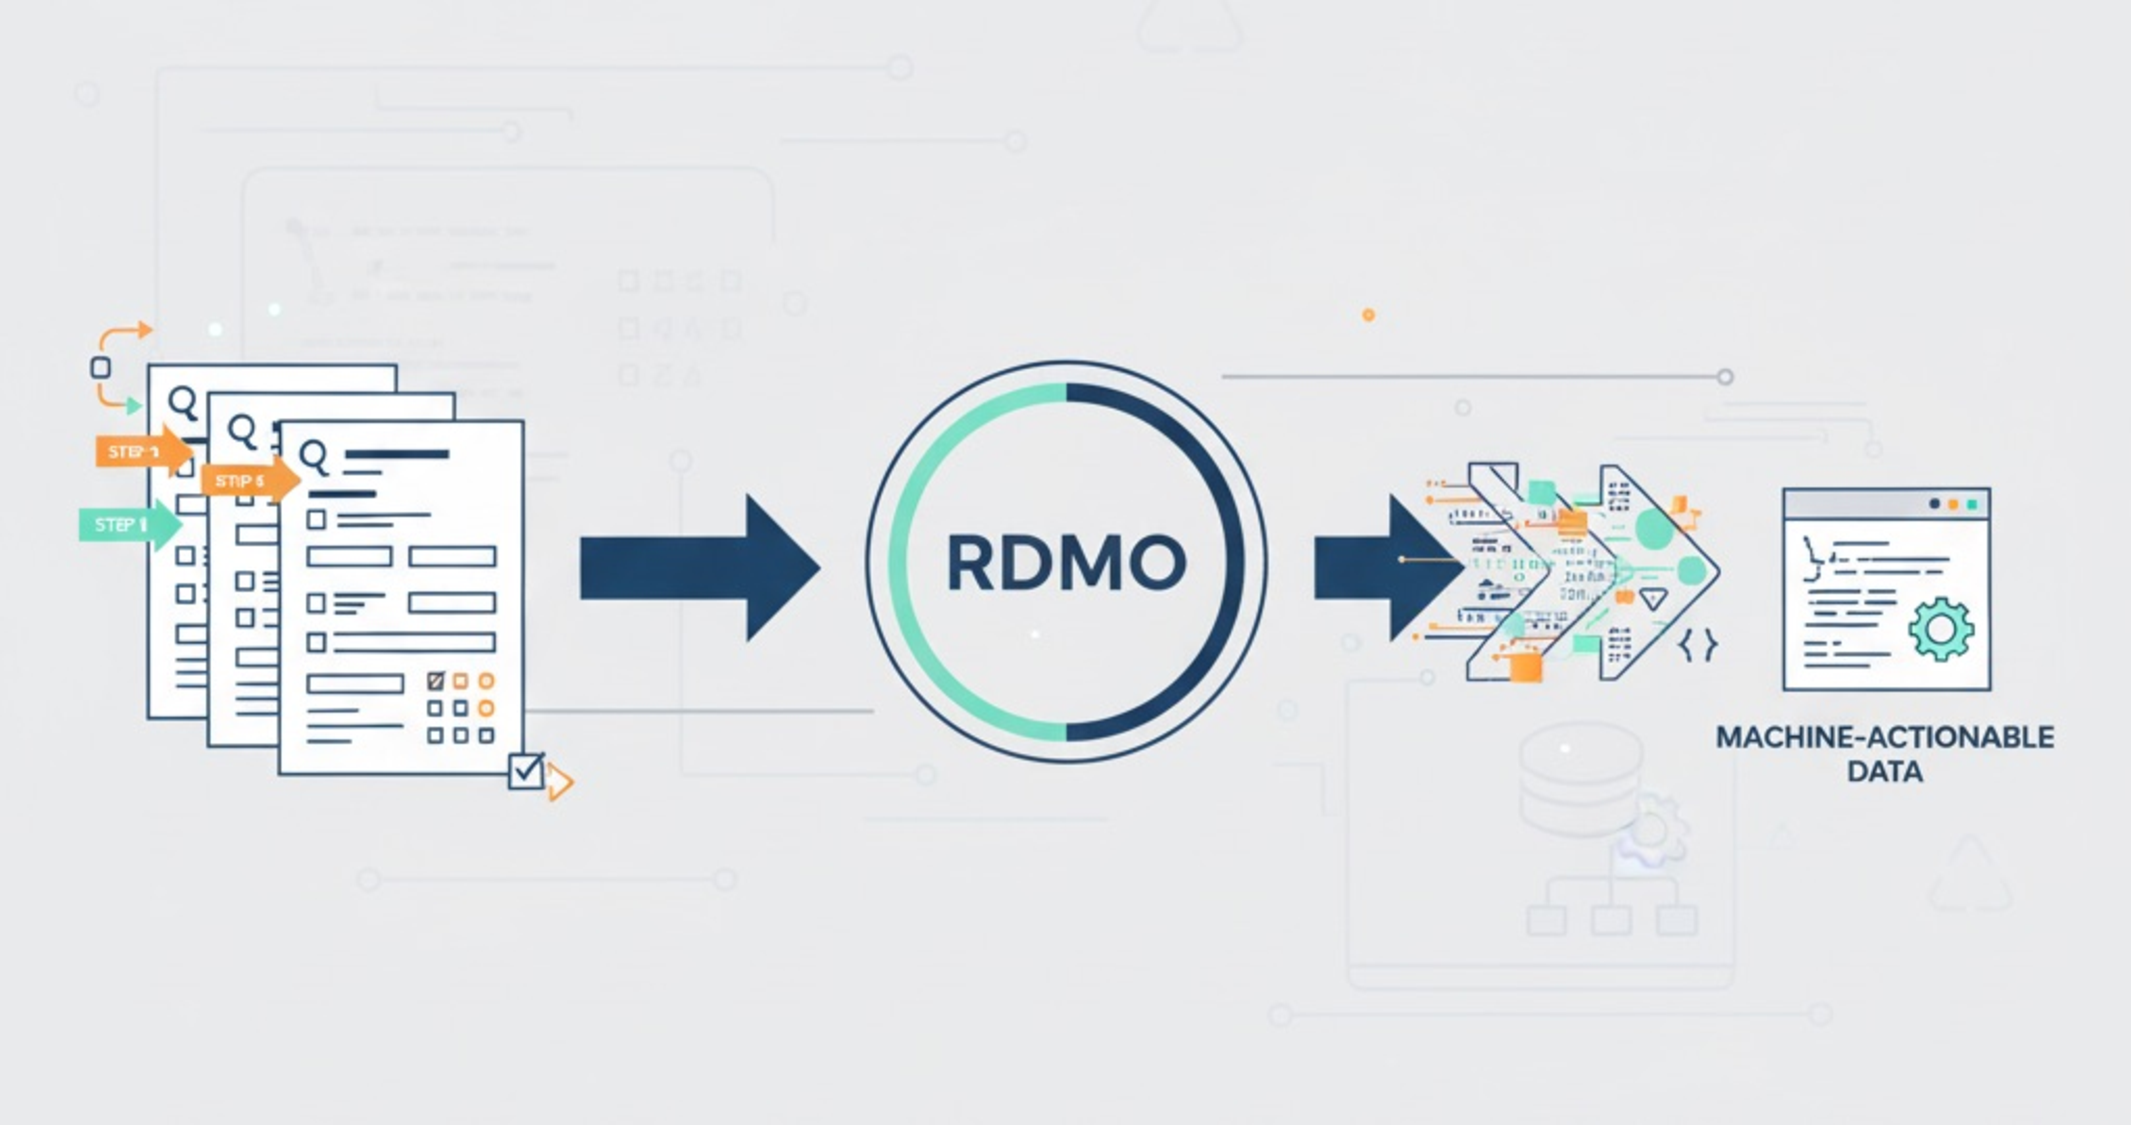
\includegraphics[width=0.32\textwidth]{figs/fig_d1p2/d1p2_01-blueprint}
            \captionof{figure}{A DMP is the blueprint for your research data.}
        \end{center}
    \end{frame}
}

\begin{frame}{Learning Objectives (2.1)}
    \begin{itemize}
        \item \textbf{Define} the four core elements of the FAIR acronym (Refresher).
        \item \textbf{Identify} the specific RDMO question categories (e.g. \emph{Metadata}, \emph{Documentation}, \emph{Long-term Preservation}) that correspond directly to each of the four FAIR principles.
    \end{itemize}
\end{frame}

\begin{frame}{Theory: What is RDMO?}{Module 2.1: Identify}
    \begin{columns}
        \column{.74\textwidth}
        The \textbf{Research Data Management Organiser (RDMO)} is a tool to support the systematic planning, implementation, and management of research data.
        \pause
        \begin{itemize}
            \item It's a "smart questionnaire."
            \item It guides you through the questions funders (like DFG) want answered.
            \item It generates a human-readable and machine-readable DMP.
            \item It is hosted by KIT!
        \end{itemize}
        
        \column{.36\textwidth}
        \begin{center}
            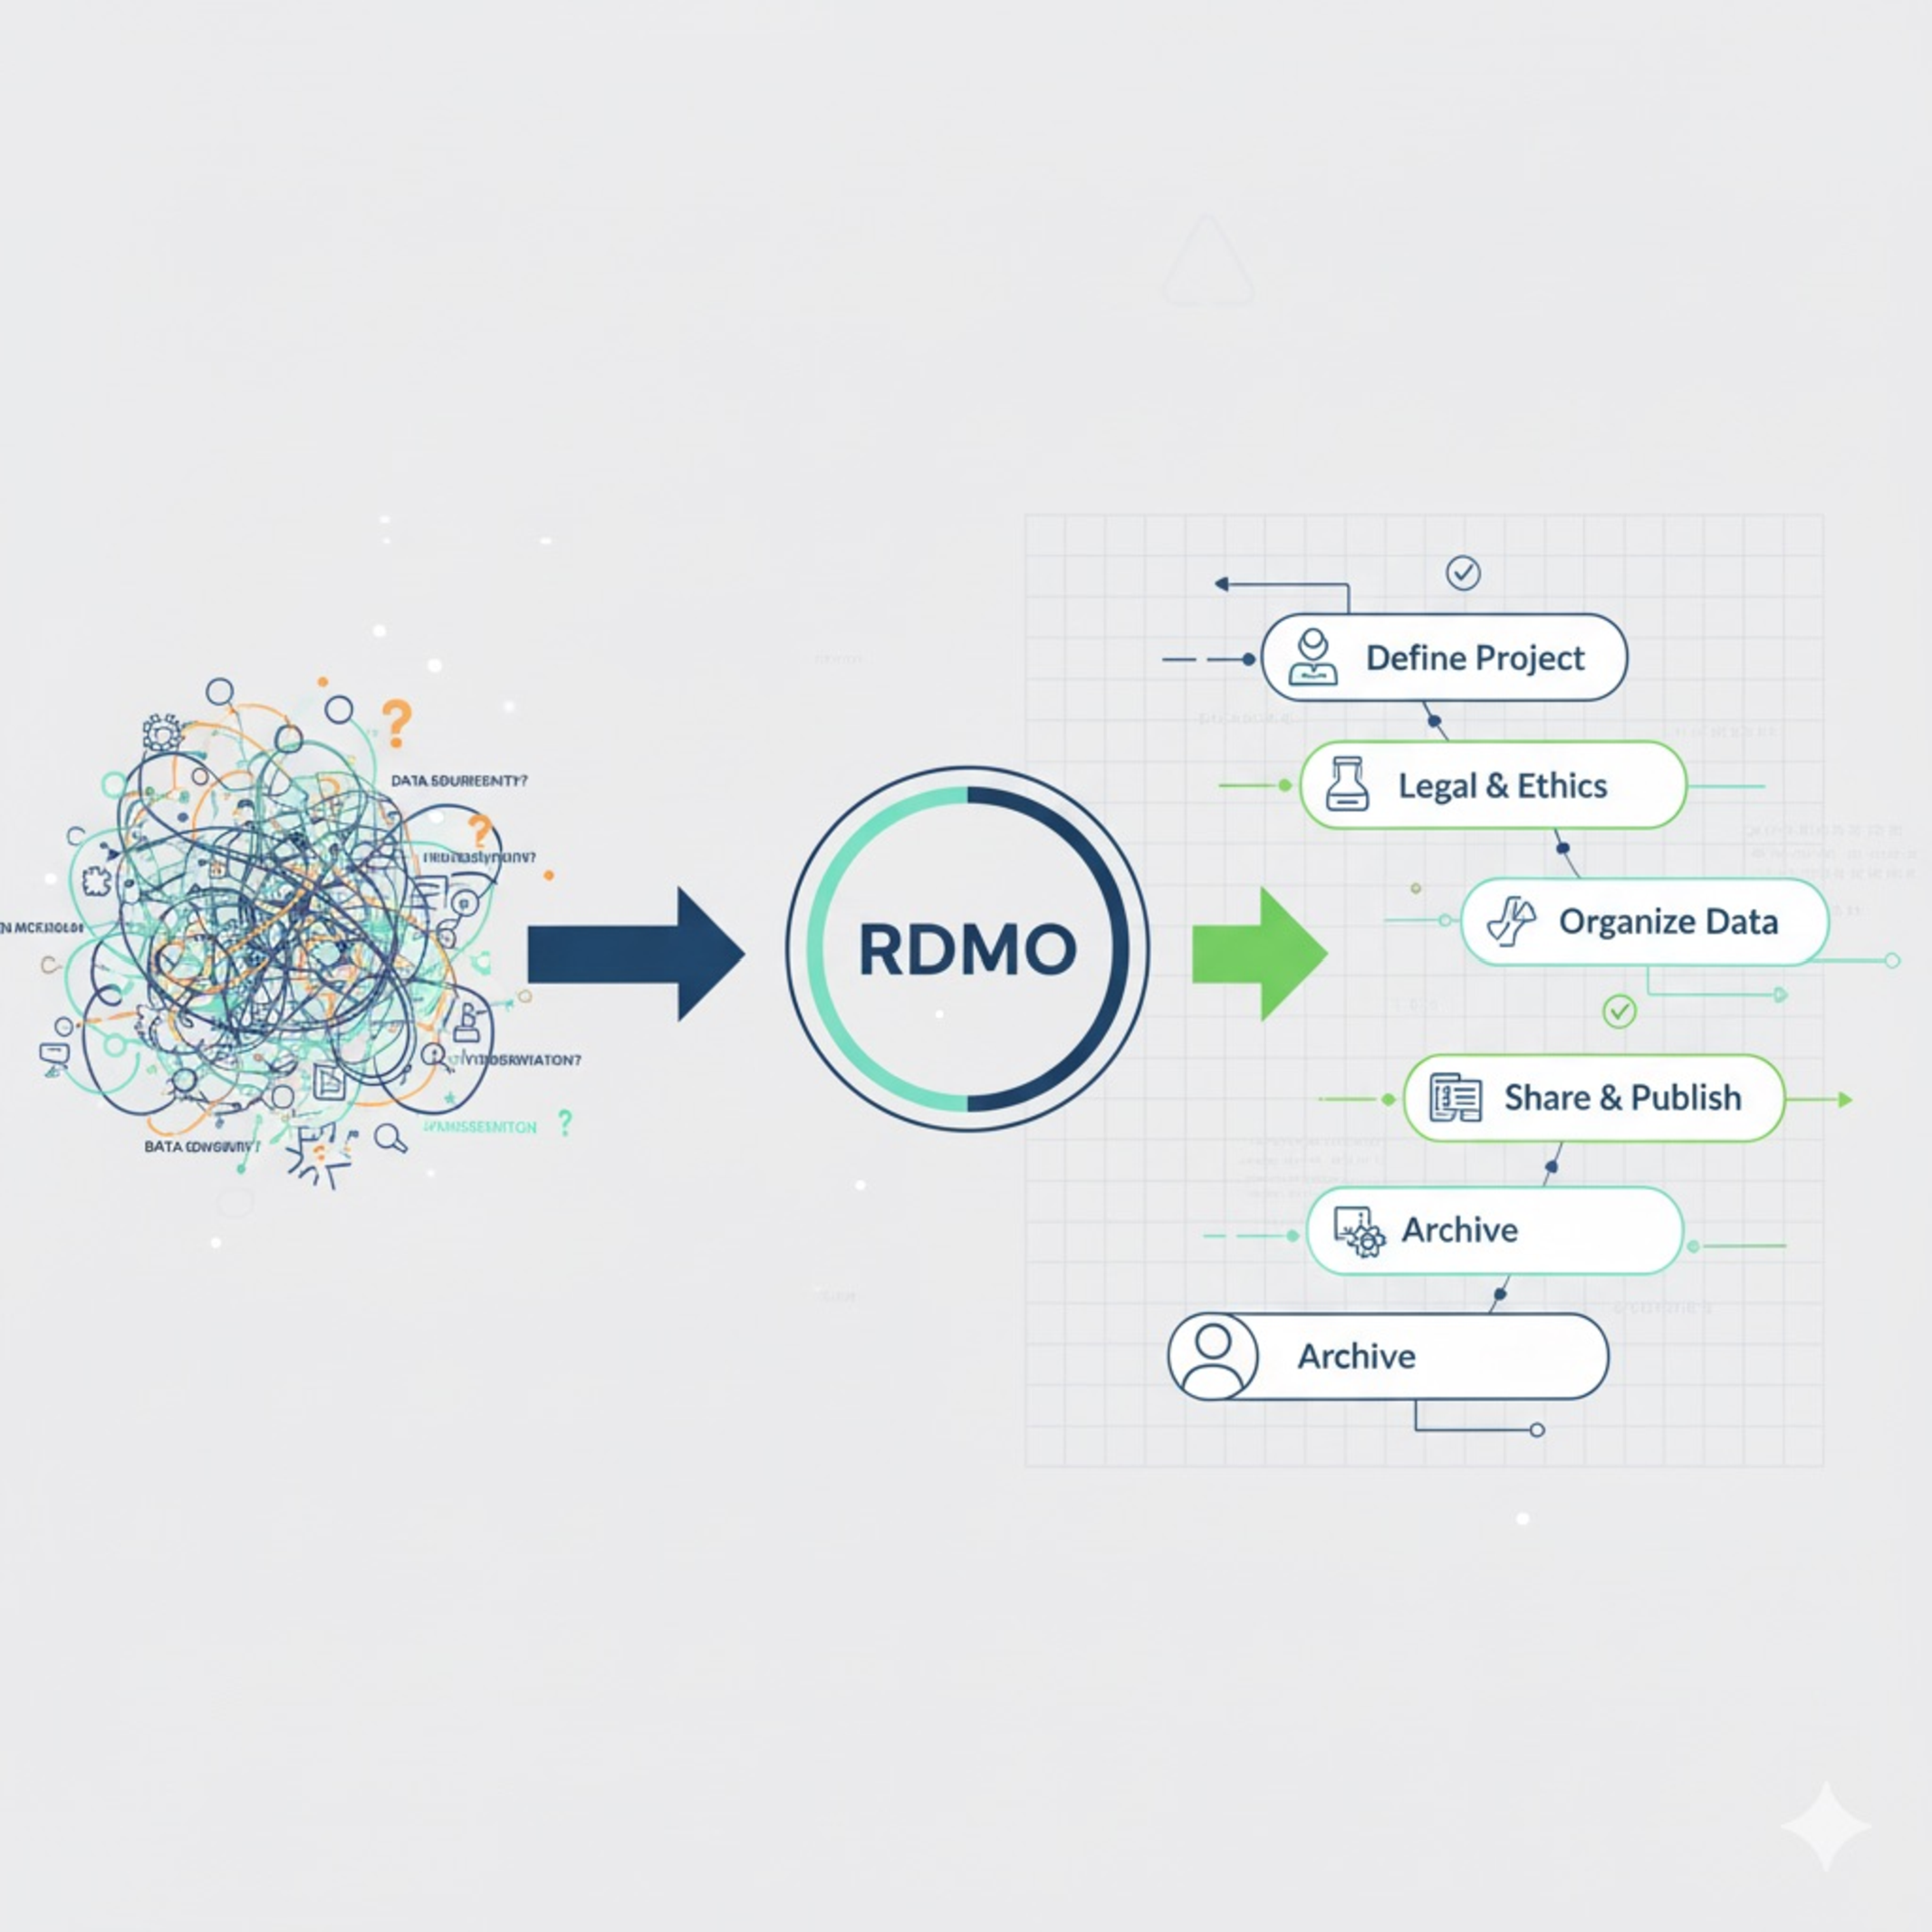
\includegraphics[width=.8\textwidth]{figs/fig_d1p2/d1p2_02-path}
        \end{center}
        \captionof{figure}{RDMO turns chaos into a structure}
    \end{columns}
\end{frame}

\begin{frame}{Concept: Mapping FAIR to RDMO}{Module 2.1: Identify}
    RDMO is structured around the RDM lifecycle, which maps directly to FAIR.
    
    \begin{itemize}
        \item \textbf{To be 'Findable' (F)...}
        \pause
        \item \textit{RDMO asks about:} "Project \& Data," "PIDs," "Repository."
        \pause
        \item \textbf{To be 'Accessible' (A)...}
        \pause
        \item \textit{RDMO asks about:} "Access \& Re-use," "Legal \& Ethical."
        \pause
        \item \textbf{To be 'Interoperable' (I)...}
        \pause
        \item \textit{RDMO asks about:} "Metadata," "Vocabularies," "Formats."
        \pause
        \item \textbf{To be 'Reusable' (R)...}
        \pause
        \item \textit{RDMO asks about:} "Documentation," "Licensing," "Quality."
    \end{itemize}
\end{frame}

\begin{frame}{Interactive: RDMO Treasure Hunt}{Module 2.1: Practice}
    \begin{block}{Activity: Log into RDMO (10 min)}
        \textbf{Task:} Log into the KIT RDMO instance. Create a new dummy project (use the "DFG" template).\\
        \pause
        \textbf{Challenge:} \textbf{Identify} the \textit{exact question} in RDMO that asks...
        \begin{itemize}
            \item How you will license your data ('R')?
            \item What metadata standard will you use ('I')?
            \item If your data will have a PID ('F')?
        \end{itemize}
        \pause
        \textbf{Goal:} \textbf{Identify} how RDMO is structured around FAIR. \\
        \textbf{URL:} \href{https://rdmorganiser.github.io}{https://rdmorganiser.github.io} \& \href{https://github.com/rdmorganiser/rdmo-docker-compose}{rdmo-docker-compose}
    \end{block}
\end{frame}

\begin{frame}{Learning Objectives (2.2)}
    \begin{itemize}
        \item \textbf{Explain} \emph{why} addressing the 'F' (Findable) principle is critical during the \textit{planning} phase.
        \item \textbf{Explain} how the structured output format of the RDMO tool supports the \textbf{Interoperability} ('I') of the DMP itself.
    \end{itemize}
\end{frame}

\begin{frame}{Theory: Why 'Findable' is a Planning Task}{Module 2.2: Explain}
    \begin{columns}
        \column{.64\textwidth}
        You can't make data "findable" \textit{after} the project is over. It's too late.
        \pause
        \begin{itemize}
            \item \textbf{Planning for 'F'} means deciding \textit{before you collect data}:
            \pause
            \item \textbf{Where} will it be published? (e.g., KITOpen)
            \item \textbf{What} is the PID strategy? (e.g., We will get a DOI)
            \item \textbf{How} will it be described? (e.g., We will use Dublin Core)
        \end{itemize}
        \pause
        If you don't plan for this, you end up with data on a hard drive that nobody (not even you) can find.
        
        \column{.36\textwidth}
        \begin{center}
            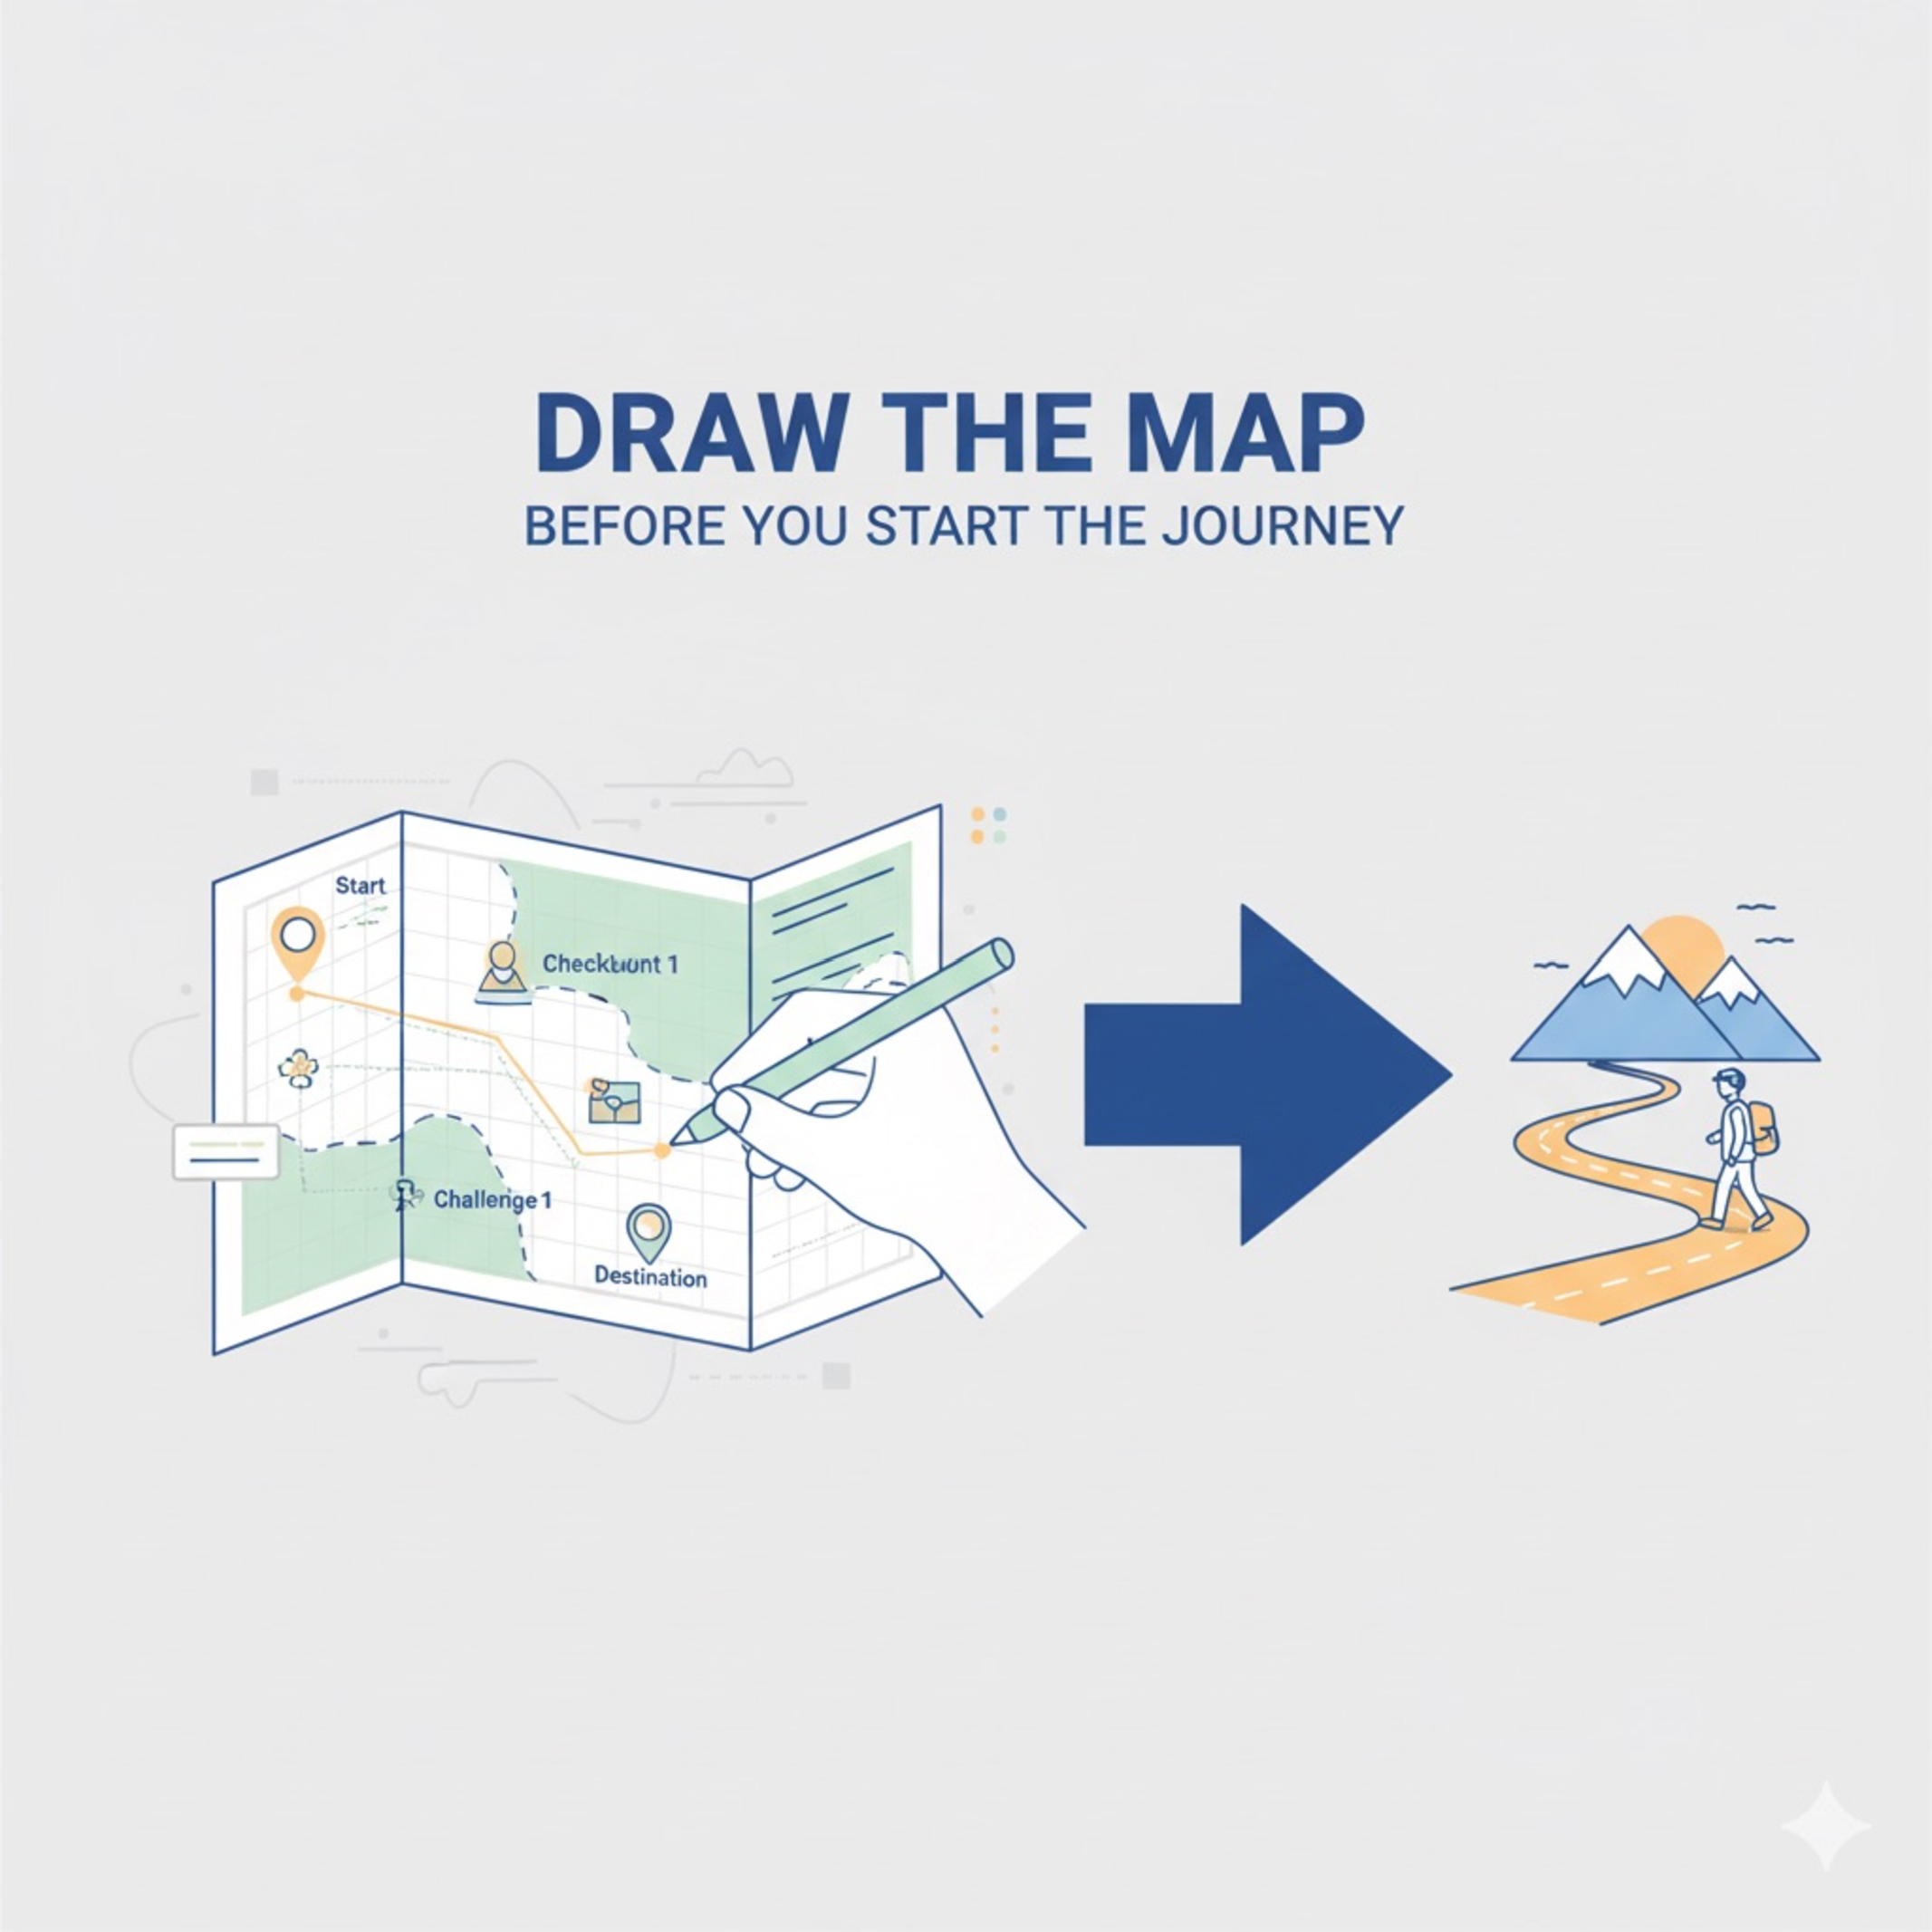
\includegraphics[width=.64\textwidth]{figs/fig_d1p2/d1p2_03-map}
       
        \end{center}
        \captionof{figure}{Draw the map \textit{before} you start the journey}
    \end{columns}
\end{frame}

\begin{frame}{Theory: RDMO for Interoperability ('I')}{Module 2.2: Explain}
    The DMP from RDMO isn't just a text document. It's a structured, machine-readable database entry.
    
    \begin{block}{The 'I' of the DMP Itself}
        You can \textbf{export} your DMP from RDMO in formats like:
        \begin{itemize}
            \item XML
            \item JSON
            \item etc. (RDMO-Instance dependant)
            \pause
            \item This means your \emph{plan} is now interoperable. It can be automatically read by funders (DFG), repositories (KITOpen), or other project management tools.
            \pause
            \item This is "FAIR for your DMP."
        \end{itemize}
    \end{block}
\end{frame}

\begin{frame}{Interactive: The "Why" of Planning}{Module 2.2: Practice}
    \begin{block}{Group Discussion (10 min)}
        \textbf{Scenario:} A researcher says, "I'm too busy doing research to write a DMP. I'll document my data when I'm finished."
        \pause
        \textbf{Task:}
        \begin{itemize}
            \item \textbf{Explain} to this researcher why this is a bad idea, using the 'F' (Findable) principle.
            \pause
            \item \textbf{Explain} how spending 2 hours on RDMO now will save them 20 hours later.
        \end{itemize}
    \end{block}
\end{frame}

\begin{frame}{Learning Objectives (2.3)}
    \begin{itemize}
        \item \textbf{Determine} the appropriate persistent identifier (e.g. DOI, Handle, ARK) to be used for the planned dataset.
        \item \textbf{Determine} and input the required \textbf{Persistent Identifier (PID) strategy} into the RDMO questionnaire.
    \end{itemize}
\end{frame}

\begin{frame}{Theory: The PID Landscape}{Module 2.3: Determine}
    A Persistent Identifier (PID) is a long-lasting reference to a digital object.
    
    \begin{columns}
        \column{.5\textwidth}
        \begin{block}{Common PIDs}
            \begin{itemize}
                \item \textbf{DOI (Digital Object Identifier):} Most common for publications and datasets. Excellent for citation.
                \item \textbf{Handle:} The system that DOIs are built on.
                \item \textbf{ARK (Archival Resource Key):} Common in libraries and archives.
                \item \textbf{ORCID:} A PID for \emph{people}.
            \end{itemize}
        \end{block}
        
        \column{.5\textwidth}
        \begin{block}{Your Strategy}
            For 99\% of researchers at Helmholtz, the strategy is simple:
            \pause
            "I will deposit my data in a repository (like KITOpen) that will mint a \textbf{DOI} for me."
            \pause
            Your job is not to \emph{create} the DOI, but to \emph{plan} on getting one.
        \end{block}
    \end{columns}
\end{frame}

\begin{frame}{Concept: Why Not Just Use a URL?}{Module 2.3: Determine}
    %% \begin{center}
    %%     \includegraphics[width=0.6\textwidth]{example-image-b}
    %%     \captionof{figure}{A URL is an address. A PID is a name.}
    %% \end{center}
    
    \begin{itemize}
        \item A standard URL (`http://my-lab.kit.edu/data.zip`) is \textbf{not persistent}.
        \item What happens when the website is redesigned? The server is changed? The researcher leaves?
        \item $\rightarrow$ \textbf{Link Rot!} The link is broken. The data is lost.
        \pause
        \item A \textbf{PID} (like a DOI) points to a \textit{resolver} (e.g., doi.org), which then redirects to the \textit{current} URL. If the URL changes (e.g., KITOpen moves servers), the repository updates the resolver. The DOI never changes.
    \end{itemize}
\end{frame}

\begin{frame}{Interactive: Your PID Strategy}{Module 2.3: Practice}
    \begin{block}{Workshop: Fill in the DMP (10 min)}
        \textbf{Task:} Go back to your draft RDMO plan.
        \pause
        \begin{enumerate}
            \item Find the section on "PIDs" or "Identifiers."
            \item \textbf{Determine} your PID strategy.
            \item \textbf{Input} your strategy.
        \end{enumerate}
        \pause
        \textbf{Example Answer:} "We will publish the final dataset in KITOpen to obtain a DOI. We will use this DOI in all publications that cite the data. Internal datasets will be identified using the HMC naming convention."
    \end{block}
\end{frame}

\begin{frame}{Learning Objectives (2.4)}
    \begin{itemize}
        \item \textbf{Distinguish} between an \emph{open} license (CC-BY) and a \emph{restrictive} license (CC-BY-NC-ND).
        \item \textbf{Justify} the selection of a specific \textbf{data access restriction model} (e.g., under embargo) in RDMO.
    \end{itemize}
\end{frame}

\begin{frame}{Theory: The License Spectrum}{Module 2.4: Distinguish}
    A license is the legal tool that makes data \textbf{Reusable ('R')}.
    
    \begin{block}{Creative Commons (CC) Licenses \href{https://creativecommons.org/share-your-work/cclicenses/}{$\therefore$}}
        \begin{itemize}
            \item \textbf{CC0 (Public Domain):} No rights reserved. The best for data!
            \pause
            \item \textbf{CC-BY (Attribution):} Anyone can use it, as long as they cite you. \textbf{(Recommended)}
            \pause
            \item \textbf{CC-BY-SA (ShareAlike):} They must also share their new work under CC-BY-SA.
            \pause
            \item \textbf{CC-BY-NC (Non-Commercial):} Cannot be used for commercial purposes. (Restricts 'R'!)
            \pause
            \item \textbf{CC-BY-ND (No-Derivatives):} Cannot be changed. (e.g., can't combine it with other data. Kills 'R'!)
        \end{itemize}
    \end{block}
\end{frame}

\begin{frame}{Theory: Access Model vs. License}{Module 2.4: Justify}
    These are two different things!
    
    \begin{itemize}
        \item \textbf{License:} What can people \emph{legally} do with your data \textit{if} they have it? (e.g., CC-BY)
        \pause
        \item \textbf{Access Model:} \textit{Who} can get the data in the first place?
        \begin{itemize}
            \item \textbf{Open Access:} Everyone.
            \item \textbf{Embargoed:} Open, but only \textit{after} a certain date (e.g., 1 year after publication).
            \item \textbf{Restricted:} Only specific people (e.g., collaborators) can access it after application.
            \item \textbf{Closed:} No one can access it.
        \end{itemize}
    \end{itemize}
    \pause
    \begin{block}{Key Idea}
        You can have an \textbf{Open License} (CC-BY) on \textbf{Restricted Data}. This means "If I approve your access, you are then free to use this data as long as you cite me."
    \end{block}
\end{frame}

\begin{frame}{Interactive: Debate - Access vs. Restriction}{Module 2.4: Practice}
    \begin{block}{Group Debate (15 min)}
        \textbf{Scenario:} Your data is publicly funded (DFG) but contains potentially patentable information.
        \pause
        \begin{columns}
            \column{.5\textwidth}
            \textbf{Group 1: Argue for...}
            \begin{itemize}
                \item Open Access
                \item CC-BY License
            \end{itemize}
            (Hint: DFG requirements, fast science)
            
            \column{.5\textwidth}
            \textbf{Group 2: Argue for...}
            \begin{itemize}
                \item Embargoed Access
                \item Restrictive License
            \end{itemize}
            (Hint: KIT tech transfer, patents)
        \end{columns}
        \pause
        \textbf{Goal:} \textbf{Justify} your data access restriction model.
    \end{block}
\end{frame}

\begin{frame}{Learning Objectives (2.5)}
    \begin{itemize}
        \item \textbf{Justify} the selection of a discipline-specific metadata standard over a general standard.
        \item \textbf{Appraise} a draft DMP against the DFG "Checklist for Handling of Research Data."
    \end{itemize}
\end{frame}

% \begin{frame}{Theory: General vs. Domain Standards}
%     \frametitle{Module 2.5: Justify}
%     \begin{columns}
%         \column{.5\textwidth}
%         \begin{block}{General Standard (e.g., Dublin Core)}
%             \begin{itemize}
%                 \item \textbf{Fields:} Creator, Title, Date, Publisher...
%                 \item \textbf{Pro:} Simple, universal. Good for 'F' and 'A'.
%                 \item \textbf{Con:} Can't describe \emph{what the data is}.
%                 \item \textbf{Metaphor:} A general library card catalog.
%             \end{itemize}
%         \end{block}
%         
%         \column{.5\textwidth}
%         \begin{block}{Domain Standard (e.g., OME-XML)}
%             \begin{itemize}
%                 \item \textbf{Fields:} `MicroscopeModel`, `LensMagnification`, `\texttt{Exposure_Time}`...
%                 \item \textbf{Pro:} Richly descriptive. Essential for 'I' and 'R'.
%                 \item \textbf{Con:} Complex, only used by experts.
%                 \item \textbf{Metaphor:} A specialized medical chart.
%             \end{itemize}
%         \end{block}
%     \end{columns}
%     \pause
%     \textbf{Justification:} "We will use Dublin Core for general findability on KITOpen, but we will \emph{also} include a `\texttt{metadata_ome.xml}` file for domain-specific reusability."
% \end{frame}

\begin{frame}{Concept: The DFG Checklist}{Module 2.5: Appraise}
    %% \begin{center}
    %%     \includegraphics[width=0.4\textwidth]{example-image-c}
    %%     \captionof{figure}{The DFG Checklist is your evaluation rubric.}
    %% \end{center}
    
    The DFG provides a "Checklist for Handling of Research Data" in its proposals. This is the list the reviewers will use to \textbf{appraise} your plan.
    \pause
    \begin{block}{Key DFG Checklist Items}
        \begin{itemize}
            \item "What data will be collected?"
            \item "What metadata standards will be used?"
            \item "Who is responsible for the data?"
            \item "How will the data be archived for 10 years?"
            \item "What costs are associated with this?"
        \end{itemize}
    \end{block}
\end{frame}

\begin{frame}{Interactive: Peer Review Your DMP}{Module 2.5: Practice}
    \begin{block}{Peer Review (15 min)}
        \textbf{Task:} Swap your draft RDMO plan (or the link) with a partner.
        \pause
        \textbf{Review:} \textbf{Appraise} your partner's DMP using the DFG Checklist.
        \pause
        \begin{itemize}
            \item Can you find the answer to "What metadata standard will be used?"
            \item Is their plan for 'Reusability' (licenses, documentation) clear?
            \item Give one piece of constructive feedback.
        \end{itemize}
        \pause
        \textbf{Goal:} \textbf{Appraise} a draft DMP and help improve it.
    \end{block}
\end{frame}

\begin{frame}{Learning Objectives (2.6)}
    \begin{itemize}
        \item \textbf{Develop} a comprehensive DMP section for the 'A' (Accessible) principle.
        \item \textbf{Generate} a complete, funder-compliant DMP for a research proposal using the RDMO tool.
    \end{itemize}
\end{frame}

\begin{frame}{Theory: Sub-Principles of 'Accessible'}{Module 2.6: Develop}
    'Accessible' is more than just "it's on the web."
    
    \begin{itemize}
        \item \textbf{A1:} (Meta)data are retrievable by their identifier using a standardised communications protocol.
        \item \textit{Your DMP Entry:} "Data will be deposited in KITOpen, which provides retrieval via HTTP and assigns a DOI."
        \pause
        \item \textbf{A1.1:} The protocol is open, free, and universally implementable.
        \item \textit{Your DMP Entry:} "The chosen protocol is HTTP(S), which is open."
        \pause
        \item \textbf{A1.2:} The protocol allows for an authentication and authorisation procedure, where necessary.
        \item \textit{Your DMP Entry:} "%For open data, no authentication is needed. For restricted data, 
        KITOpen manages authorisation."
        \pause
        \item \textbf{A2:} Metadata are accessible, even when the data are no longer available.
        \item \textit{Your DMP Entry:} "The repository (KITOpen) guarantees metadata persistence even if the data is removed."
    \end{itemize}
\end{frame}

\begin{frame}{Interactive: Finalize Your DMP}{Module 2.6: Practice}
    \begin{block}{Workshop (20 min)}
        \textbf{Task:} Go back to your RDMO plan one last time.
        \pause
        \begin{enumerate}
            \item Review your answers for 'Access' (Module 2.4) and 'Metadata' (Module 2.5).
            \pause
            \item Ensure every question has a clear, concise, and specific answer. (e.g., change "a repository" to "KITOpen").
            \pause
            \item Click the "Export" button and look at the generated document.
        \end{enumerate}
        \pause
        \textbf{Goal:} \textbf{Generate} a complete, funder-compliant DMP.
    \end{block}
\end{frame}

\begin{frame}{Module 2: Summary}
    \begin{itemize}
        \item The \textbf{DMP} is the central \emph{planning} document for FAIR.
        \item \textbf{RDMO} is the tool that guides us through this plan.
        \item We must plan for \textbf{PIDs ('F')}, \textbf{Licenses ('R')}, \textbf{Access ('A')}, and \textbf{Standards ('I')} from Day 1.
        \item A good DMP is the \textbf{blueprint} for your research and the key to your funding proposal.
    \end{itemize}
    \vfill
    \begin{center}
        \textbf{End of Part 2}
    \end{center}
\end{frame}

% ===================================================================
% PART 3: Integrating RDM in Research Operation
% ===================================================================

\section{Operations: RDM in Practice}
{
    \setbeamertemplate{background canvas}{
        
\includegraphics[width=\paperwidth,height=\paperheight]{figs/background_white.png}
    }
    \begin{frame}[plain]{Day 1 - Part 3: RDM in Research Operations}
        %% %% \frametitle{12:15 - 13:00}
        \begin{block}{Module 3 Goal}
            A plan is useless without action. We will learn to integrate RDM (ELNs, Git, Pipelines) into our \textbf{daily research operations}.
        \end{block}
       %% \begin{center}
       %%     \includegraphics[width=0.6\textwidth]{example-image-a}
       %%     \captionof{figure}{From blueprint (DMP) to construction (Operation).}
       %% \end{center}
    \end{frame}
}

\begin{frame}{Learning Objectives (3.1)}
    \begin{itemize}
        \item \textbf{List} the mandatory data records (e.g., metadata, raw data, scripts) required for project closure.
        \item \textbf{Identify} the mandatory metadata fields (e.g., sample ID, instrument ID) to be logged in an \textbf{ELN} upon acquisition.
    \end{itemize}
\end{frame}

\begin{frame}{Theory: The "Project Closure" Package}{Module 3.1: List}
    When your project ends, you must archive a "research package" that ensures Reusability and meets DFG's 10-year rule.
    
    \begin{block}{Mandatory Records for Archiving}
        \begin{itemize}
            \item \textbf{1. Raw Data:} The original, unaltered files from the instrument.
            \pause
            \item \textbf{2. Processed Data:} The final, clean data used for figures.
            \pause
            \item \textbf{3. Metadata:} The `README` or `metadata.xml` that describes everything.
            \pause
            \item \textbf{4. Scripts:} The code (e.g., Python, R, Matlab) used to get from Raw to Processed.
            \pause
            \item \textbf{5. Documentation:} The ELN export, codebook, or lab journal.
        \end{itemize}
    \end{block}
\end{frame}

\begin{frame}{Theory: The ELN at Acquisition}{Module 3.1: Identify}
    To build that archive, you must capture metadata \emph{at the moment of acquisition} in your \textbf{Electronic Lab Notebook (ELN)}.
    
    %% \begin{columns}
        %% \column{.5\textwidth}
        %% \includegraphics[width=\textwidth]{example-image-b}
        
        %% \column{.5\textwidth}
        \begin{block}{Mandatory ELN Fields \cite{zb_med-informationszentrum_lebenswissenschaften_electronic_2021}}
            Your ELN template for a new experiment should \textbf{force} you to enter:
            \begin{itemize}
                \item `\texttt{experiment\_ID}`, `\texttt{operator\_name}`
                \item `\texttt{date\_time}` (timestamp), `\texttt{instrument\_ID}`
                \item `\texttt{sample\_ID(s)}`, `\texttt{project\_name}`
                \item `\texttt{hypothesis}` (Why are you doing this?)
            \end{itemize}
        \end{block}
    %% \end{columns}
    \pause
    If you don't record this \emph{now}, it is lost forever. This is the core of operational data integrity.
\end{frame}

\begin{frame}{Interactive: Design Your ELN Template}{Module 3.1: Practice}
    \begin{block}{Activity: Your ELN Template (10 min)}
        \textbf{Task:} You are setting up a new ELN (e.g., \href{https://demo-kadi4mat.iam.kit.edu}{https://demo-kadi4mat.iam.kit.edu}). You are creating a template for a "standard experiment" in your field.
        \pause
        \textbf{Brainstorm:}
        \begin{itemize}
            \item \textbf{List} 5-10 \textbf{mandatory metadata fields} you must capture.
            \item \textbf{Identify} the \textit{one} field that is most often forgotten, but causes the most problems later.
        \end{itemize}
        \pause
        \textbf{Goal:} \textbf{Identify} mandatory fields for your ELN.
        \href{https://demo-kadi4mat.iam.kit.edu/templates/8}{$\therefore$}
    \end{block}
\end{frame}

\begin{frame}{Learning Objectives (3.2)}
    \begin{itemize}
        \item \textbf{Summarise} the differences in data access controls and their impact on operational security.
        \item \textbf{Illustrate} how connecting an \textbf{Instrument Registry} to the ELN automatically fulfils 'F' and 'I'.
    \end{itemize}
\end{frame}

\begin{frame}{Theory: Access Controls in Operation}{Module 3.2: Summarise}
    Access controls are not just for publishing. They are for \emph{operational security} during the project.
    
    \begin{itemize}
        \item \textbf{Problem:} Your "in-progress" data is often your most sensitive asset.
        \pause
        \item \textbf{Risk 1 (Too Open):} Data on a shared drive with no access control. A student from another group accidentally deletes it. (Integrity failure!)
        \pause
        \item \textbf{Risk 2 (Too Closed):} Data on your personal laptop. If you get sick, your team cannot continue working. (Operational failure!)
        \pause
        \item \textbf{Solution:} Use \textbf{role-based access}.
        \begin{itemize}
            \item `Project\_Leader`: Read/Write
            \item `PhD\_Student`: Read/Write
            \item `Master\_Student`: Read-Only (on raw data)
            \item `External\_Collaborator`: Read-Only (on processed data)
        \end{itemize}
    \end{itemize}
\end{frame}

\begin{frame}{Theory: The Instrument Registry}{Module 3.2: Illustrate}
    %% \begin{center}
    %%     \includegraphics[width=0.8\textwidth]{example-image-c}
    %%     \captionof{figure}{Manual vs. Automated ELN Entry}
    %% \end{center}
    
    \begin{columns}
        \column{.4\textwidth}
            \begin{block}{Manual Way (Low 'I')}
            \textbf{ELN Field:} `instrument\_name` \\
            \textbf{You type:} "The new microscope in room 205" \\
            \pause
            \textbf{Problem:} This is free-text. It's not machine-readable. It's not interoperable. \\
        \end{block}
        
        \column{.6\textwidth}
        \begin{block}{Automated Way (High 'I')}
            An \textbf{Instrument Registry} is a database of all lab equipment. \\
            \pause
            \textbf{ELN Field:} `instrument\_ID` \\
            \textbf{You select:} `HMC-KIT-Microscope-047` \\
            \pause
            \textbf{Result:} Your data is now \emph{linked} to that instrument's entire history (calibration, model, etc.). \\
            This is \textbf{Interoperability ('I')} and \textbf{Findability ('F')}!
        \end{block}
    \end{columns}
\end{frame}

\begin{frame}{Interactive: Your Security Workflow}{Module 3.2: Practice}
    \begin{block}{Discussion (10 min)}
        \textbf{Task:} \textbf{Summarise} the access controls on your current project's "in-progress" data.
        \pause
        \begin{itemize}
            \item Who has access?
            \item Is it too open or too closed?
            \item How does this impact your operational security?
        \end{itemize}
        \pause
        \textbf{Illustration:}
        \begin{itemize}
            \item \textbf{Illustrate} (by drawing a diagram) how connecting your lab's instrument list (even a simple Excel file) to your ELN would improve your data's 'I' and 'R' value.
        \end{itemize}
    \end{block}
    ex. \href{https://sms.atmohub.kit.edu}{Sensor Management System} delivers PIDs like :
    https://hdl.handle.net/21.11157/b88fe935-2072-4106-8aca-f008e2feab48
\end{frame}

\begin{frame}{Learning Objectives (3.3)}
    \begin{itemize}
        \item \textbf{Execute} the process of version control (e.g., using Git) on analysis scripts, ensuring \textbf{traceability}.
        \item \textbf{Configure} a \textbf{message broker} (e.g., Kafka) to route data streams from an instrument.
    \end{itemize}
\end{frame}

\begin{frame}{Theory: Version Control for Traceability}{Module 3.3: Execute}
    \begin{columns}
        \column{.36\textwidth}
        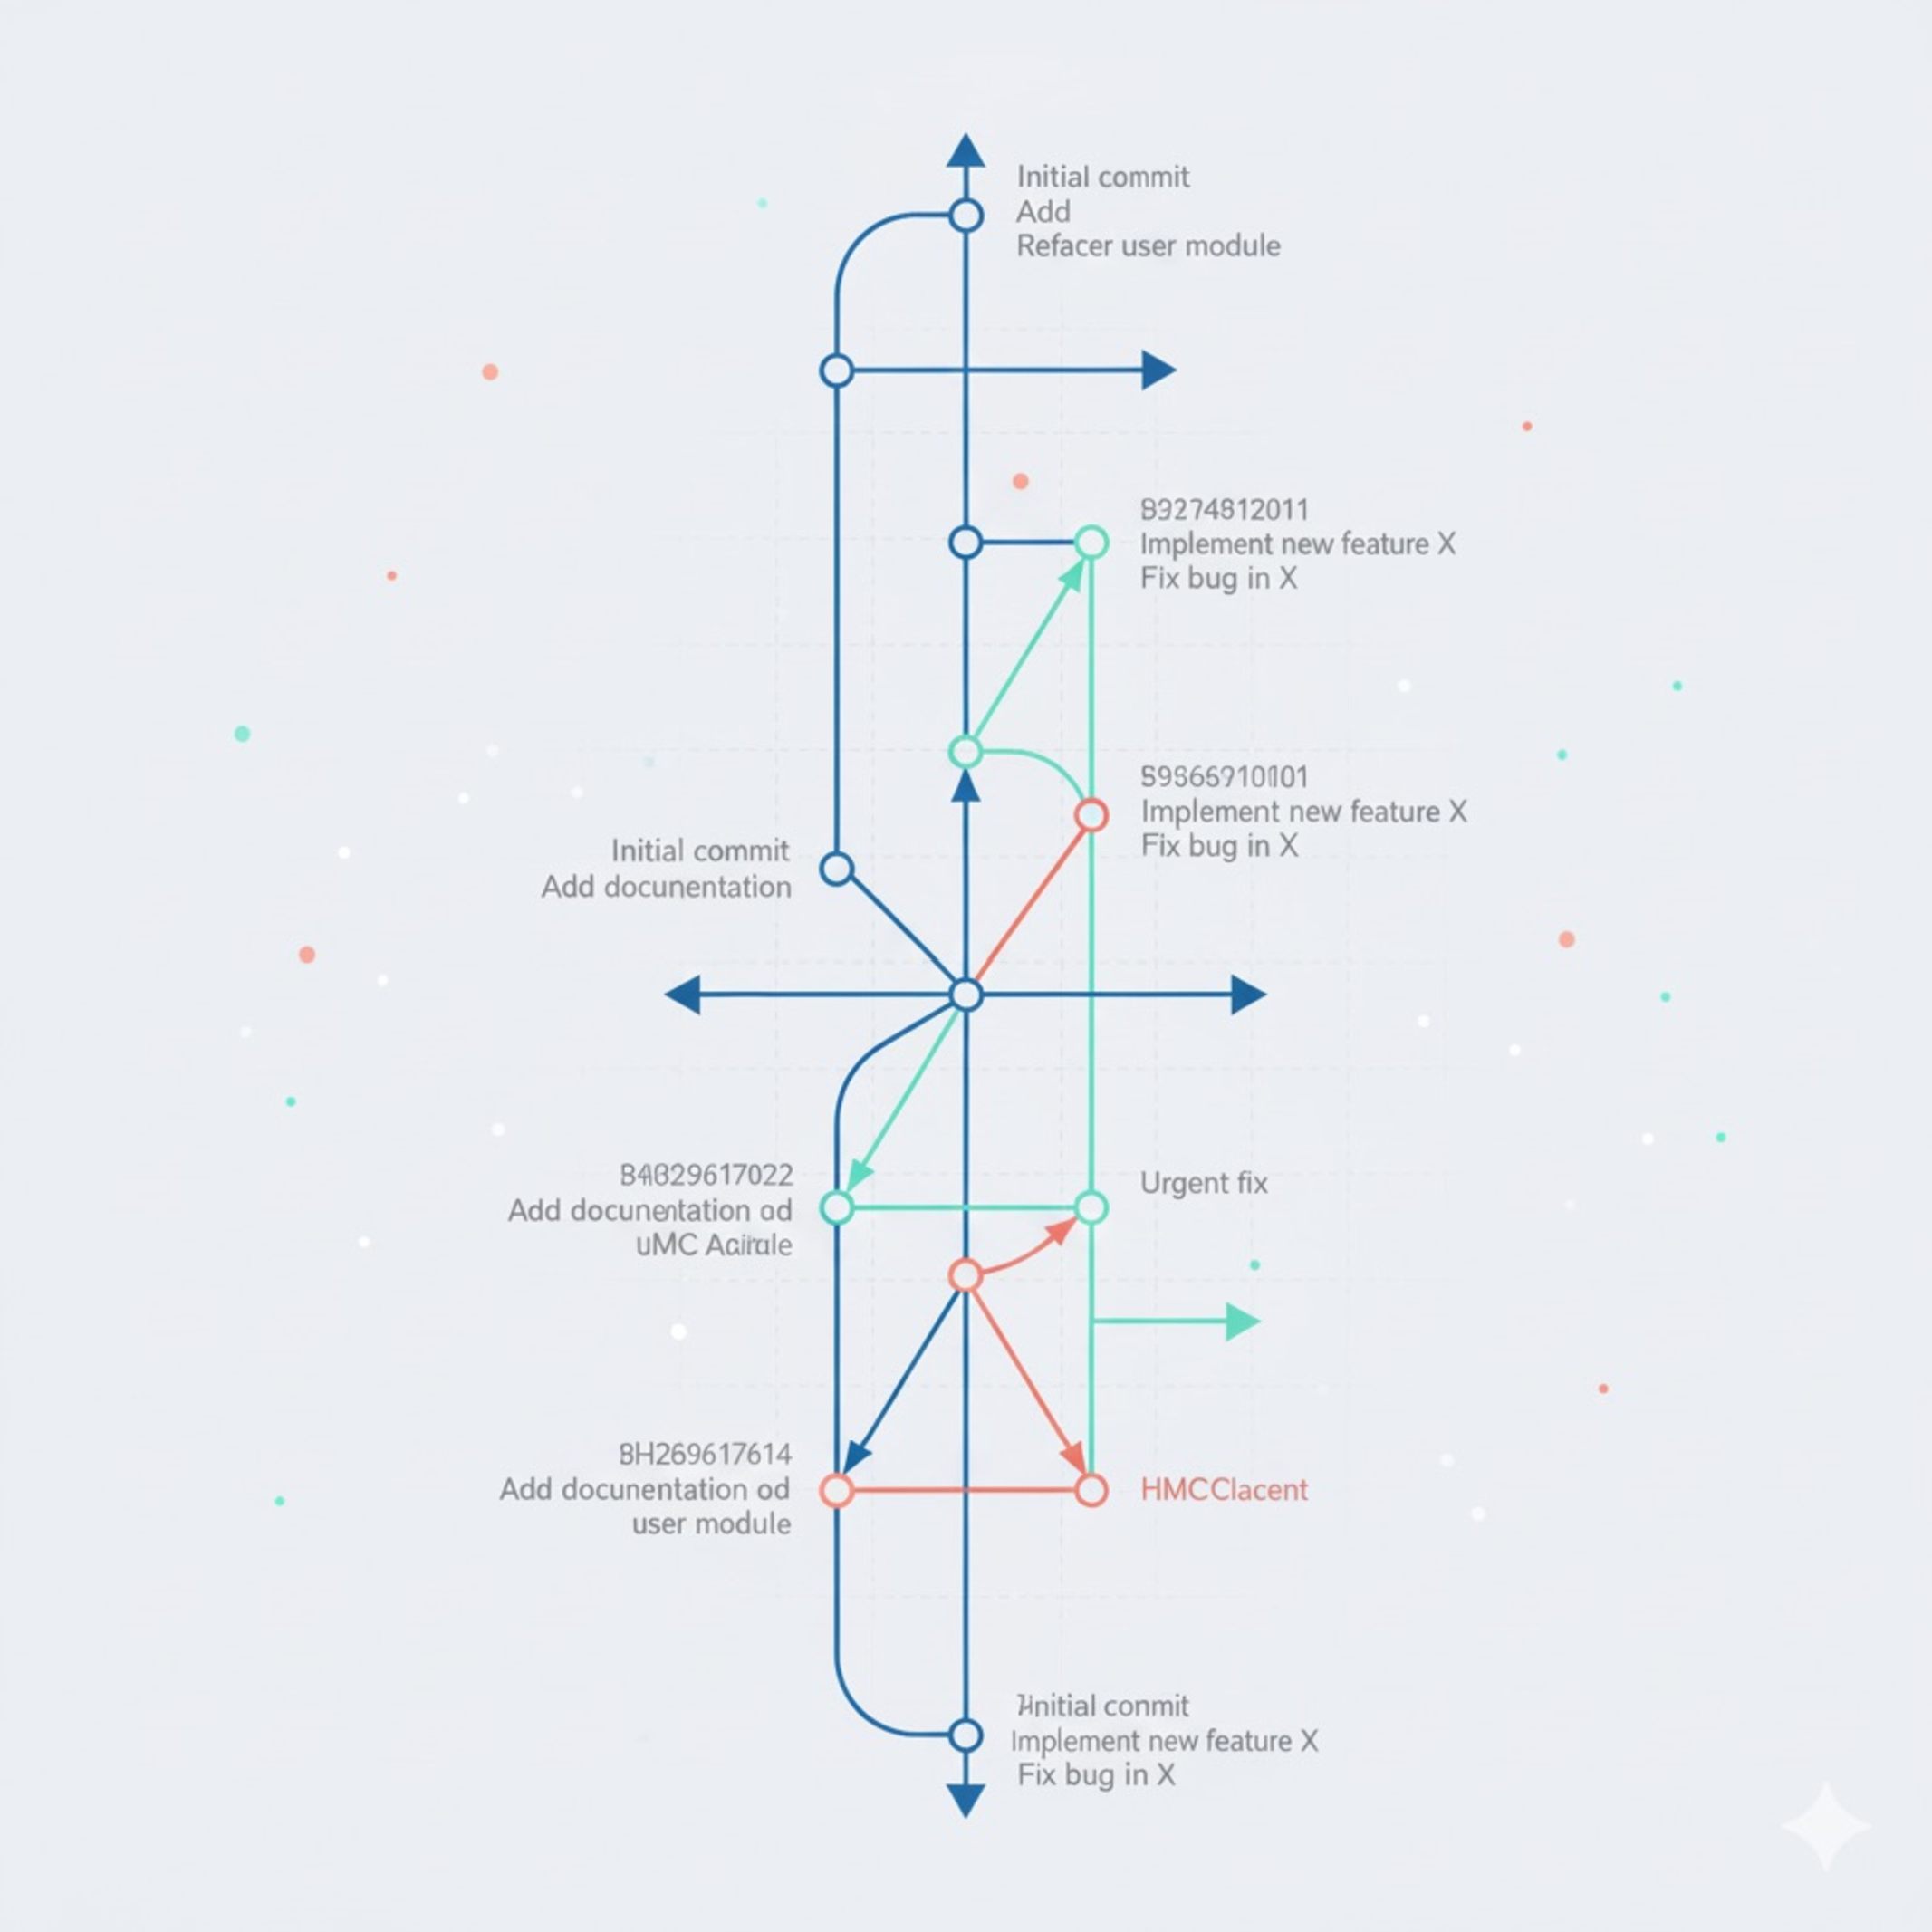
\includegraphics[width=\textwidth]{figs/fig_d1p3/d1p3_01-log}
        \captionof{figure}{Git provides a full history of changes.}
        
        \column{.64\textwidth}
        Your analysis script (e.g., `analyse.py`) is \textbf{data}. It's the recipe that turns raw data into a result. \\
        \pause
        \textbf{Problem:}
        `analyse\_v1.py`
        `analyse\_v2\_final.py`
        `analyse\_v2\_final\_FOR\_REAL.py` \\
        \pause
        This is a \textbf{traceability nightmare}. You no longer know which script made which figure. \\ % This is a \textbf{Data Integrity} failure. \\
        \pause
        \textbf{Solution: Git}
        \begin{itemize}
            \item `git commit -m "Added new filtering step"`
            \item `git commit -m "Fixed bug in axis label"`
        \end{itemize}
        Now you have 100\% traceability.
    \end{columns}
\end{frame}

\begin{frame}{Theory: The Message Broker}{Module 3.3: Configure}
    %% \begin{center}
    %%     \includegraphics[width=0.8\textwidth]{example-image-b}
    %%     \captionof{figure}{A message broker acts as a central post office for data.}
    %% \end{center}
    
    A \textbf{Message Broker} (like Kafka, RabbitMQ, or MQTT) is a tool that routes data streams.
    \pause
    \begin{itemize}
        \item \textbf{Instrument} $\rightarrow$ "Publishes" data to a topic (e.g., `lab/microscope/raw\_data`)
        \pause
        \item \textbf{Broker} $\rightarrow$ Receives the data.
        \pause
        \item \textbf{ELN} $\rightarrow$ "Subscribes" to the topic and automatically ingests the data.
        \item \textbf{Archive} $\rightarrow$ \textit{Also} subscribes and makes a backup.
    \end{itemize}
    \pause
    This is the gold standard for automated, high-integrity data capture.
\end{frame}

\begin{frame}{Interactive: Hands-On Traceability}{Module 3.3: Practice}
    \begin{block}{Workshop (20 min)}
        This is a hands-on session.
    \end{block}
    %% \begin{columns}
    %%     \column{.5\textwidth}
        \begin{block}{Track 1: Version Control (Git)}
            \textbf{Goal:} \textbf{Execute} version control.
            \pause
            \begin{itemize}
                \item Create a folder.
                \item Create `script.py`.
                \item Run: `git init`
                \item Run: `git add .`
                \item Run: `git commit -m "Initial commit"`
            \end{itemize}
            You just ensured traceability!
        \end{block}

       %% \column{.5\textwidth}
       %% \begin{block}{Track 2: Message Broker (Demo)}
       %%     \textbf{Goal:} \textbf{Configure} a broker.
       %%     \pause
       %%     \begin{itemize}
       %%         \item (Live Demo)
       %%         \item 1. Start a simple MQTT broker.
       %%         \item 2. Run a "sensor" script that publishes data.
       %%         \item 3. Run a "logger" script that subscribes and prints the data.
       %%     \end{itemize}
       %% \end{block}
    %% \end{columns}
\end{frame}

\begin{frame}{Learning Objectives (3.4)}
    \begin{itemize}
        \item \textbf{Differentiate} between data annotation methods for \emph{qualitative} vs. \emph{quantitative} data.
        \item \textbf{Troubleshoot} a data pipeline error by \textbf{analysing} message broker logs.
    \end{itemize}
\end{frame}

\begin{frame}{Theory: Data Annotation Methods}{Module 3.4: Differentiate}
    Annotation (metadata) is not one-size-fits-all.
    
    \begin{columns}
        \column{.5\textwidth}
        \begin{block}{Quantitative Data (Numbers)}
            \textbf{Data:} `10.5`
            \textbf{Annotation Needs:}
            \begin{itemize}
                \item \textbf{Vocabularies:} What is it? (e.g., `PATO:0000125` - "temperature" see \href{https://www.ebi.ac.uk/ols4/}{OLS})
                \item \textbf{Units:} What unit? (e.g., `UO:0000027` - "degree Celsius")
                \item \textbf{Precision:} `+/- 0.05`
            \end{itemize}
            \textbf{Goal:} Consistency, machine-readability.
        \end{block}
        
        \column{.5\textwidth}
        \begin{block}{Qualitative Data (Text/Image)}
            \textbf{Data:} "The sample showed significant degradation..."
            \textbf{Annotation Needs:}
            \begin{itemize}
                \item \textbf{Coding Schemas:} What does "significant degradation" mean? (e.g., `Degradation\_Level\_3`)
                \item \textbf{Context:} Who wrote this? When?
                \item \textbf{Tags:} `\#failed\_experiment`, `\#contamination`
            \end{itemize}
            \textbf{Goal:} Context, findability, interpretation.
        \end{block}
    \end{columns}
\end{frame}

\begin{frame}{Theory: Troubleshooting the Pipeline}{Module 3.4: Troubleshoot}
    %% \begin{center}
    %%     \includegraphics[width=0.7\textwidth]{example-image-a}
    %%     \captionof{figure}{Instrument $\rightarrow$ Broker $\rightarrow$ ELN}
    %% \end{center}
    
    \textbf{Problem:} The ELN is recording gibberish, but the instrument seems fine. Where is the error?
    \pause
    \begin{itemize}
        \item \textbf{Step 1:} Check the Message Broker logs. Is the data arriving at the broker correctly?
        \pause
        \item \textbf{Yes:} The data is fine. The problem is the \textbf{ELN subscriber} (Track 2). It's misinterpreting the message.
        \pause
        \item \textbf{No:} The data is not in the logs, or it's already gibberish. The problem is the \textbf{Instrument publisher} (Track 1). It's sending bad data.
    \end{itemize}
    \pause
    The broker's log is your central point for \textbf{troubleshooting}.
\end{frame}

\begin{frame}{Interactive: The Pipeline is Broken!}{Module 3.4: Practice}
    \begin{block}{Scenario (15 min)}
        \textbf{Problem:} Your ELN is recording temperatures as `25.3` (correct), but pressures as `NULL`.
        \pause
        \textbf{Logs:} The broker log shows:
        `{"topic": "lab/sensor/temp", "payload": "25.3"}`
        `{"topic": "lab/sensor/pressure", "payload": "101.3"}`
        \pause
        \textbf{Task: Analyse \& Troubleshoot}
        \begin{itemize}
            \item Is the instrument working? (Yes)
            \item Is the broker working? (Yes)
            \item What is the problem?
            \pause
            \item \textbf{Answer:} The ELN is subscribed to `lab/sensor/temp` but \emph{not} to `lab/sensor/pressure`. It's a configuration error in the subscriber.
        \end{itemize}
        \textbf{Goal:} \textbf{Troubleshoot} a pipeline error.
    \end{block}
\end{frame}

\begin{frame}{Learning Objectives (3.5)}
    \begin{itemize}
        \item \textbf{Assess} the current team workflow against the DMP.
        \item \textbf{Compare} and \textbf{evaluate} manual vs. automated data capture, justifying the superior method based on \textbf{verifiability}.
    \end{itemize}
\end{frame}

\begin{frame}{Theory: Assessing Workflow vs. DMP}{Module 3.5: Assess}
    Your DMP is your \textbf{plan}. Your workflow is your \textbf{reality}. You must \textbf{assess} reality against the plan. \\
    \pause
    \begin{block}{The "DMP Audit"}
        \textbf{Your DMP says:} "All data will be annotated with a standard vocabulary." \\
        \pause
        \textbf{Your Workflow is:} A student is typing free-text notes into the ELN. \\
        \pause
        \textbf{Result:} \textbf{Non-compliant.} You have a bottleneck. \\
        \pause
        \textbf{Solution:} You must \textbf{assess} this gap and fix it (e.g., build a drop-down list in the ELN). \\
    \end{block}
\end{frame}

\begin{frame}{Theory: Manual vs. Automated (Verifiability)}{Module 3.5: Compare}
    \textbf{Verifiability} (Data Integrity) is the ability to prove your data is correct.
    
    \begin{columns}
        \column{.5\textwidth}
        \begin{block}{Method 1: Manual Entry}
            \begin{itemize}
                \item Student reads "10.5" from screen.
                \item Student types "10.5" into Excel.
                \item \textbf{Verifiability:} Low.
                \item \textbf{Error Points:} Typo? Did they misread? Did they skip a line? You can \emph{never} be 100\% sure.
            \end{itemize}
        \end{block}
        
        \column{.5\textwidth}
        \begin{block}{Method 2: Automated Pipeline}
            \begin{itemize}
                \item Instrument sends "10.5".
                \item Broker logs "10.5".
                \item ELN records "10.5".
                \item \textbf{Verifiability:} High.
                \item \textbf{Error Points:} None (in transcription). The log \emph{proves} what the instrument sent.
            \end{itemize}
        \end{block}
    \end{columns}
    \pause
    \textbf{Justification:} The automated pipeline is superior not because it's faster, but because it is \textbf{verifiable}.
\end{frame}

\begin{frame}{Interactive: Debate - Manual vs. Automated}{Module 3.5: Practice}
    \begin{block}{Group Evaluation (10 min)}
        \textbf{Scenario:} A senior professor says, "These new automated pipelines are a black box. I trust my PhD students to write down the numbers correctly. It's how I've always done it."
        \pause
        \textbf{Task:}
        \begin{itemize}
            \item \textbf{Compare} the two methods.
            \item Form a polite, respectful argument. \textbf{Justify} why the automated pipeline is superior, using the concept of \textbf{verifiability}.
        \end{itemize}
        \pause
        \textbf{Goal:} \textbf{Evaluate} two methods.
    \end{block}
\end{frame}

\begin{frame}{Learning Objectives (3.6)}
    \begin{itemize}
        \item \textbf{Develop} a comprehensive, step-by-step \textbf{workflow diagram} that integrates automated metadata creation.
        \item \textbf{Design} a resilient, end-to-end RDM workflow for data collection.
    \end{itemize}
\end{frame}


\begin{frame}{Theory: The End-to-End Workflow}
    
    \begin{itemize}
        \item \textbf{Plan:} DMP (from RDMO)
        \item \textbf{Acquire:} Instrument + Instrument Registry
        \item \textbf{Transport:} Message Broker
        \item \textbf{Record:} ELN (with required fields)
        \item \textbf{Process:} Analysis Scripts (versioned in Git)
        \item \textbf{Publish:} Repository (KITOpen / OEP)
    \end{itemize}
\end{frame}


\begin{frame}{Theory: The End-to-End Workflow}{Module 3.6: Develop}
    Let's put all the pieces from today together.
    \begin{center}
        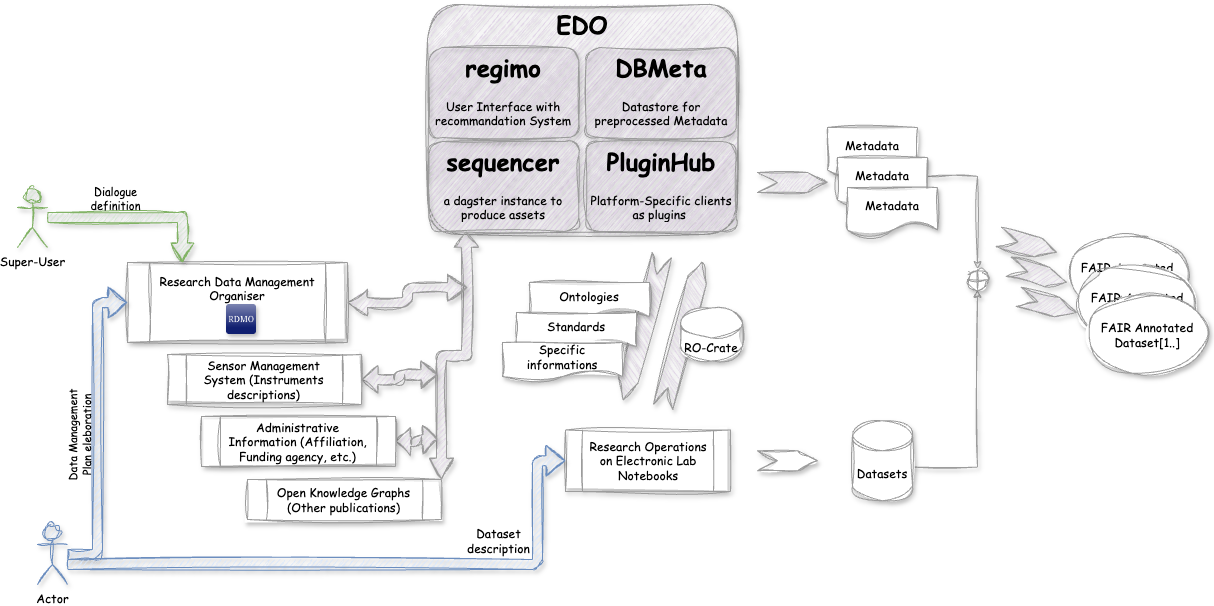
\includegraphics[width=.72\textwidth]{figs/fig_d1p3/edo_overview.png}
        \captionof{figure}{A conceptual diagram of a full RDM-integrated workflow.}
    \end{center}
\end{frame}

\begin{frame}{Interactive: Design Your Workflow}{Module 3.6: Practice}
    \begin{block}{Activity: Whiteboard Session (20 min)}
        \textbf{Task:} As a group, \textbf{design} your ideal, resilient, end-to-end RDM workflow.
        \pause
        \textbf{Instructions:}
        \begin{itemize}
            \item Draw it on a whiteboard or paper.
            \item Start with the \textbf{Instrument}.
            \item End with the \textbf{Publication} (on KITOpen/OEP).
            \item \textbf{Must Include:} Your ELN, a Message Broker, and Git.
            \item Show where metadata is created and where it flows.
        \end{itemize}
        \pause
        \textbf{Goal:} \textbf{Develop} and \textbf{Design} a comprehensive workflow diagram.
    \end{block}
\end{frame}

\begin{frame}{Module 3: Summary}
    \begin{itemize}
        \item RDM is not just planning; it's \textbf{daily operation}.
        \item \textbf{ELNs} are the core tool for capturing metadata at acquisition.
        \item \textbf{Git} ensures traceability (integrity) for your scripts.
        \item \textbf{Message Brokers} provide a verifiable, automated path from instrument to ELN.
        \item We must \textbf{assess} our real workflow against our DMP.
    \end{itemize}
    \vfill
    \begin{center}
        \textbf{End of Day 1}
    \end{center}
\end{frame}

% ===================================================================
% PART 4: Recording and Transforming Metadata, Serialisation
% ===================================================================

\section{Metadata: Serialization}

\begin{frame}{Day 2 - Part 4: Metadata Serialisation}{10:00 - 10:45}
    \begin{block}{Module 4 Goal}
        Welcome to Day 2! We will focus on the \textit{structure} and \textit{format} of metadata. It's not just \emph{what} you record, but \emph{how} you encode it.
    \end{block}
    \begin{center}
        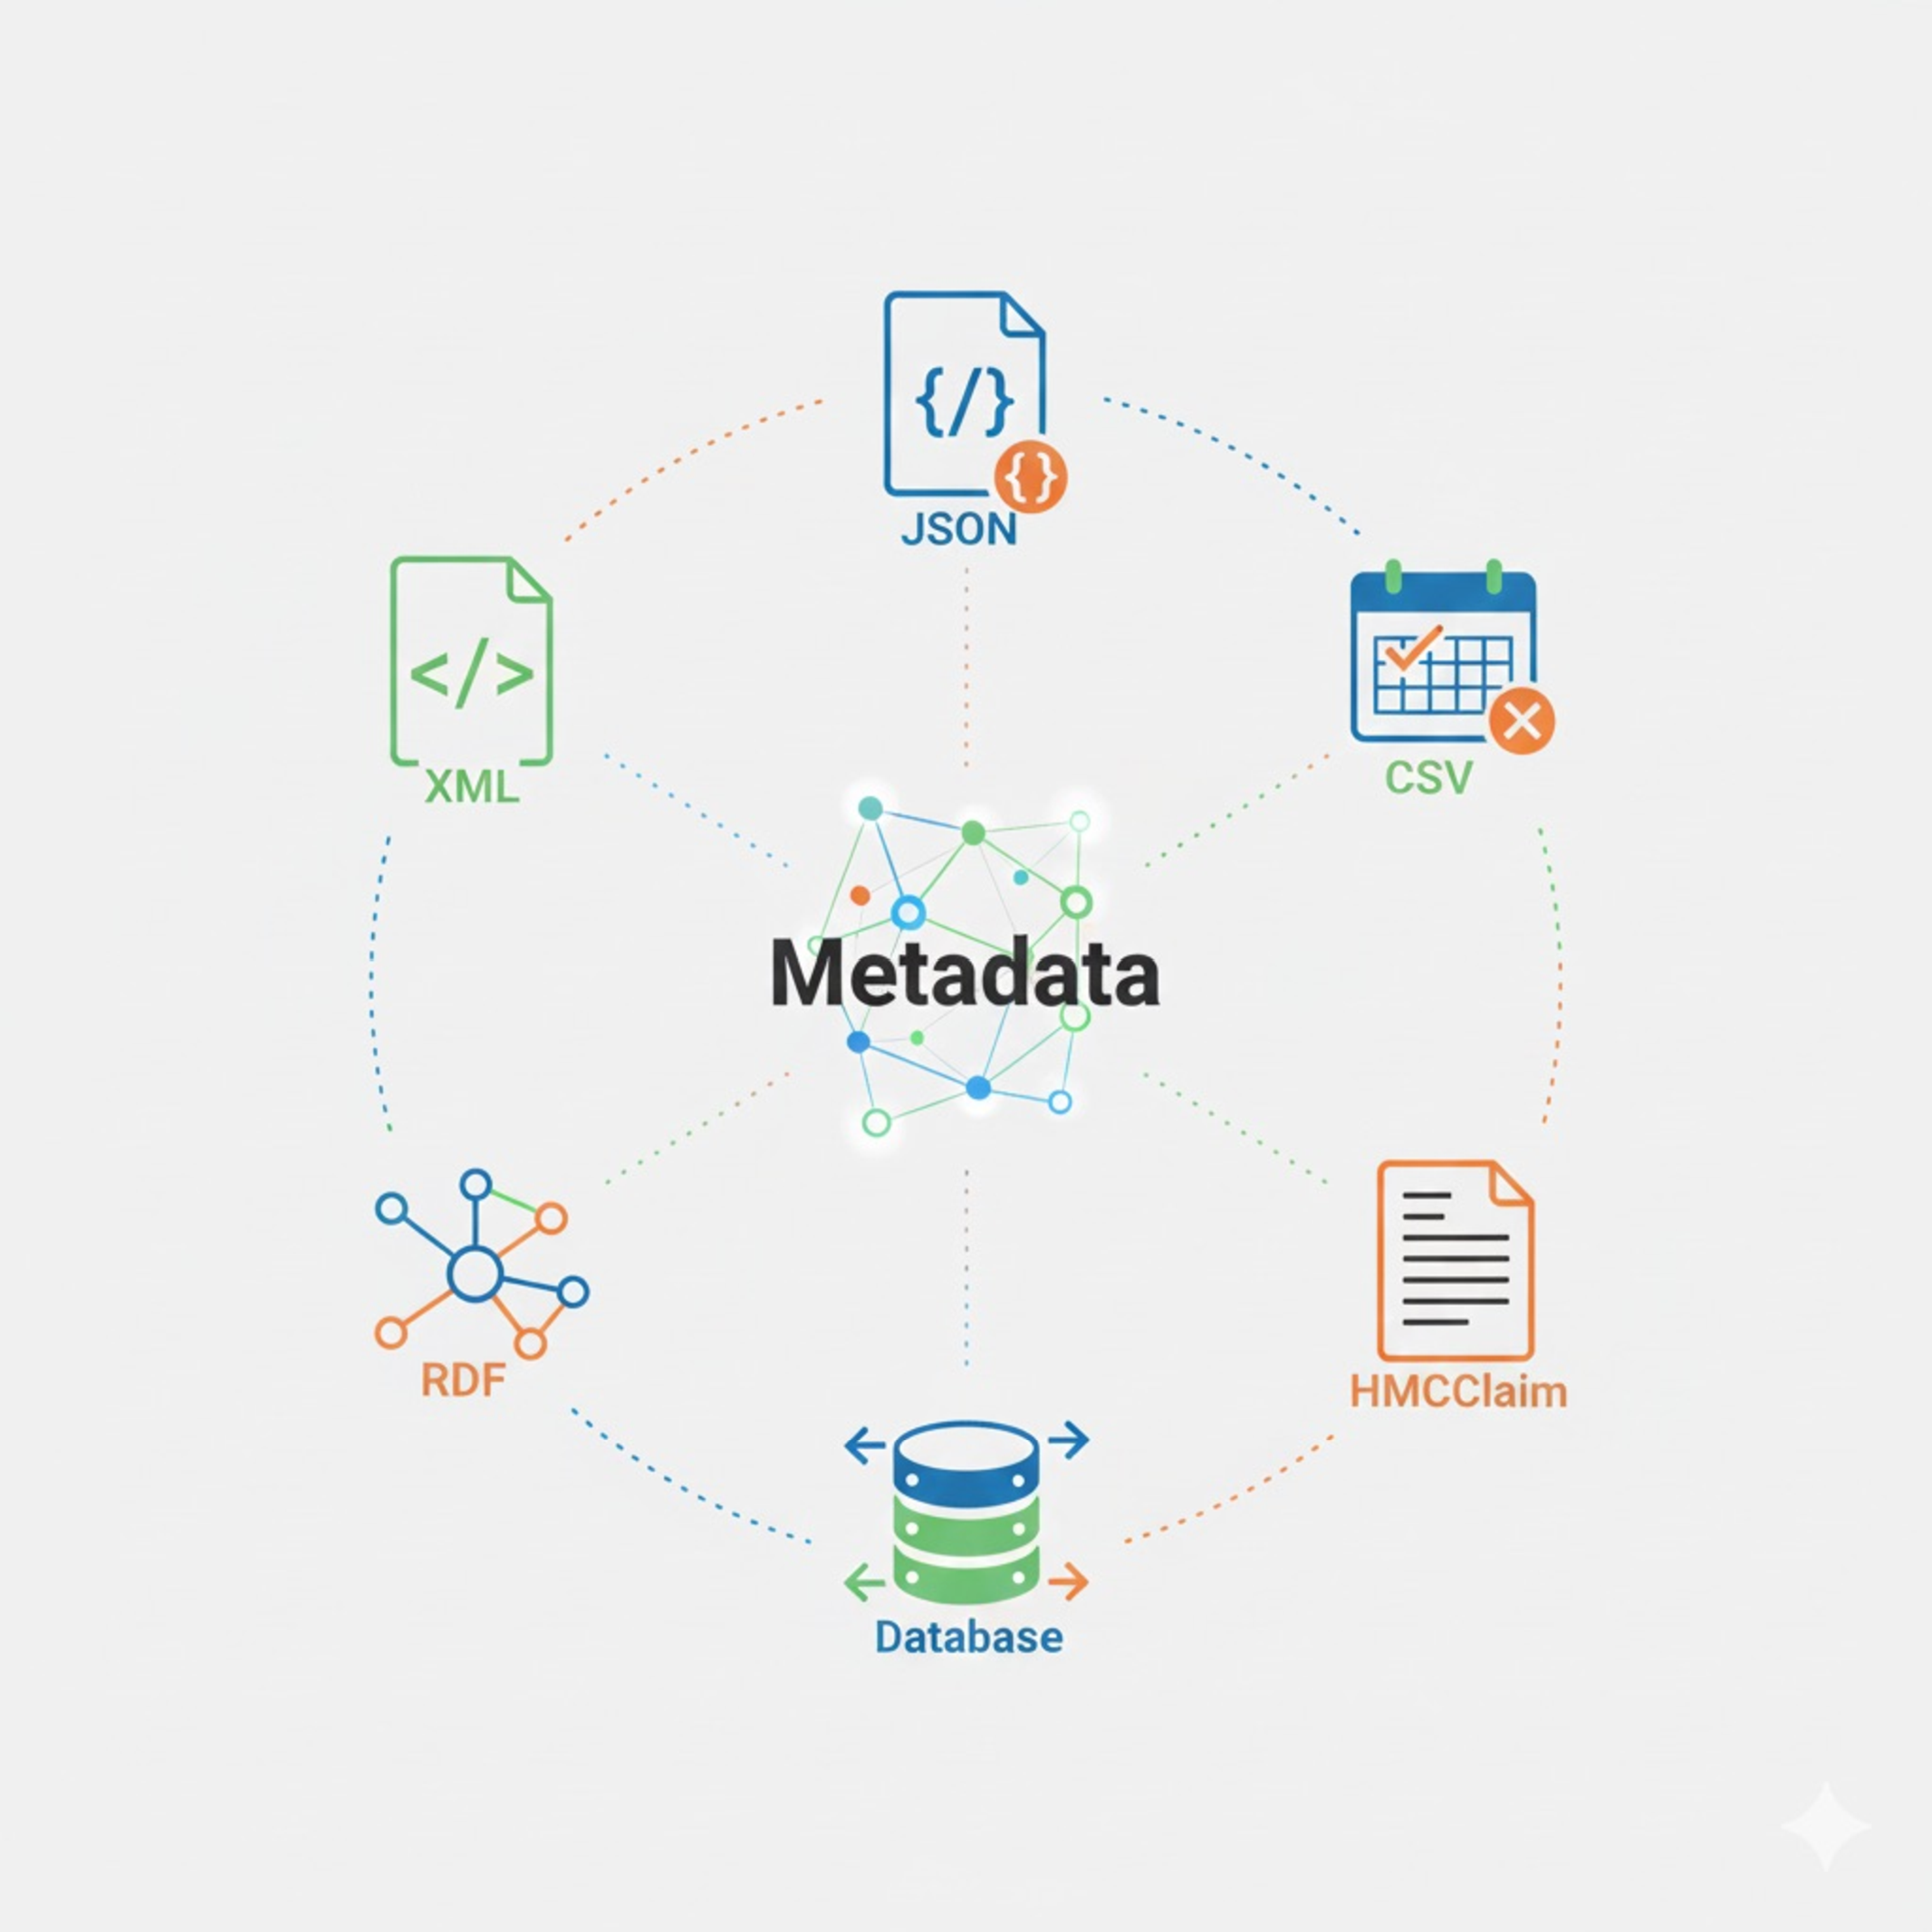
\includegraphics[width=0.32\textwidth]{figs/fig_d2p4/fig_d2p4_01-container}
        \captionof{figure}{Metadata can be stored in many different "containers" (formats).}
    \end{center}
\end{frame}

\begin{frame}{Learning Objectives (4.1)}
    \begin{itemize}
        \item \textbf{Recall} the core components of a minimal metadata standard (e.g., Dublin Core).
        \item \textbf{Recall} the structural differences between common metadata serialisation formats (XML, JSON, CSV).
    \end{itemize}
\end{frame}

\begin{frame}{Theory: Minimal Standard (Dublin Core)}{Module 4.1: Recall}
    \textbf{Dublin Core (DC)} is a "lowest common denominator" metadata standard. It provides 15 simple fields to describe \textit{anything}.
    
    \begin{block}{The 15 Dublin Core Elements}
        \begin{columns}
            \column{.32\textwidth}
            \begin{itemize}
                \item Title
                \item \textbf{Creator}
                \item Subject
                \item \textbf{Description}
                \item Publisher
            \end{itemize}
            
            \column{.32\textwidth}
            \begin{itemize}
                \item Contributor
                \item \textbf{Date}
                \item \textbf{Type}
                \item \textbf{Format}
                \item \textbf{Identifier}
            \end{itemize}
            
            \column{.32\textwidth}
            \begin{itemize}
                \item Source
                \item Language
                \item Relation
                \item Coverage
                \item \textbf{Rights} (License)
            \end{itemize}
        \end{columns}
    \end{block}
    This is the minimum you should provide for 'F' and 'R'.
\end{frame}

\begin{frame}[fragile]{Theory: Serialisation Formats}{Module 4.1: Recall}
    How do we write this metadata down?
    
    \begin{columns}
        \column{.33\textwidth}
        \begin{block}{CSV}
        \vspace{1.2ex}
            \begin{lstlisting}[language=CSV]
Title,Creator
My Data,A. Researcher
            \end{lstlisting}
            \vspace{1.2ex}
            \begin{itemize}
                \item Simple
                \item No hierarchy
            \end{itemize}
            
        \end{block}
        
        \column{.33\textwidth}
        \begin{block}{XML}
        \vspace{1.2ex}
            \begin{lstlisting}[language=XML]
<Title>My Data</Title>
<Creator>A. Researcher</Creator>
            \end{lstlisting}
            \vspace{1.2ex}
            \begin{itemize}
                \item Verbose
                \item Strict (Schemas!)
            \end{itemize}
        \end{block}
        
        \column{.33\textwidth}
        \begin{block}{JSON}
            \begin{lstlisting}[language=json]
{
  "Title": "My Data",
  "Creator": "A. Researcher"
}
            \end{lstlisting}
            \begin{itemize}
                \item Web-friendly
                \item Less strict
            \end{itemize}
        \end{block}
    \end{columns}
\end{frame}

\begin{frame}{Interactive: Format Brainstorm}
    \framesubtitle{Module 4.1: Practice}
    \begin{block}{Group Brainstorm (10 min)}
        \textbf{Task:} Let's \textbf{recall} the pros and cons of these formats.
        \begin{itemize}
            \item When would \textbf{CSV} be a \textit{good} choice for metadata?
            \pause
            \item When would \textbf{XML} be a \textit{better} choice than JSON? (Hint: Think about strict rules).
            \pause
            \item Why has \textbf{JSON} become the most popular format for web APIs?
        \end{itemize}
    \end{block}
\end{frame}

\begin{frame}{Learning Objectives (4.2)}
    \begin{itemize}
        \item \textbf{Differentiate} between \textbf{descriptive} and \textbf{technical} metadata.
        \item \textbf{Differentiate} between the role of a \textbf{metadata schema} (structure) and a \textbf{serialisation format} (encoding).
    \end{itemize}
\end{frame}

\begin{frame}{Theory: Types of Metadata}
    \framesubtitle{Module 4.2: Differentiate}
    Not all metadata is the same.
    
    \begin{columns}
        \column{.5\textwidth}
        \begin{block}{Descriptive Metadata}
            \textbf{What} the data is.
            \begin{itemize}
                \item Title
                \item Creator
                \item Abstract
                \item Keywords
            \end{itemize}
            \textbf{Purpose:} Findability, Citation. ('F', 'R')
        \end{block}
        
        \column{.5\textwidth}
        \begin{block}{Technical Metadata}
            \textbf{How} the data was made.
            \begin{itemize}
                \item `Software: Python 3.9`
                \item `Instrument: HMC-Microscope-047`
                \item `File Format: .csv`
                \item `Checksum: md5:ab...c1`
            \end{itemize}
            \textbf{Purpose:} Reusability, Validation. ('I', 'R')
        \end{block}
    \end{columns}
\end{frame}

\begin{frame}{Theory: Schema vs. Serialisation}
    \framesubtitle{Module 4.2: Differentiate}
    This is the most important concept in this module.
    
    %% \begin{center}
    %%     \includegraphics[width=0.7\textwidth]{example-image-a}
    %% \end{center}
    
    \begin{itemize}
        \item \textbf{Schema (The Blueprint):} The \textit{rules}.
        \item "You MUST have a Title. The Date MUST be in `YYYY-MM-DD` format."
        \item (e.g., Dublin Core, XSD, JSON-Schema)
        \pause
        \item \textbf{Serialisation (The Building Material):} The \textit{format} you write it in.
        \item "We will write these rules in XML."
        \item (e.g., XML, JSON, Turtle)
    \end{itemize}
    \pause
    You can use the \textbf{Dublin Core schema} and serialise it as \textbf{XML}, \textbf{JSON}, or even \textbf{CSV}.
\end{frame}

\begin{frame}{Interactive: Schema or Format?}
    \framesubtitle{Module 4.2: Practice}
    \begin{block}{Quiz (10 min)}
        I'll name a term. You tell me: \textbf{Schema (Rule)} or \textbf{Serialisation (Format)}?
        \pause
        \begin{itemize}
            \item JSON? $\rightarrow$ \textbf{Format}
            \pause
            \item Dublin Core? $\rightarrow$ \textbf{Schema}
            \pause
            \item XML? $\rightarrow$ \textbf{Format}
            \pause
            \item ISO 19115 (for Geospatial data)? $\rightarrow$ \textbf{Schema}
            \pause
            \item `metadata.csv`? $\rightarrow$ \textbf{Format}
            \pause
            \item JSON-Schema? $\rightarrow$ \textbf{Schema} (A schema for the JSON format!)
        \end{itemize}
    \end{block}
\end{frame}

\begin{frame}{Learning Objectives (4.3)}
    \begin{itemize}
        \item \textbf{Annotate} a raw dataset file by applying a selected discipline-specific metadata standard.
        \item \textbf{Annotate} a raw dataset file by applying a minimal metadata schema (Dublin Core) and exporting the result in a serialisation format (JSON).
    \end{itemize}
\end{frame}

\begin{frame}{Theory: What is Annotation?}
    \framesubtitle{Module 4.3: Annotate}
    Annotation is the act of \emph{linking} a piece of data to its metadata.
    
    \begin{block}{Example Annotation}
        \textbf{Raw Data:} `my\_experiment.csv`
        \pause
        \textbf{Annotation (in a separate JSON file):}
% \begin{lstlisting}[language=json]
% {
%   "file_name": "my_experiment.csv",
%   "dc:title": "Temperature Experiment",
%   "dc:creator": "Researcher, A.",
%   "dc:date": "2025-11-14",
%   "my_schema:instrument": "HMC-Microscope-047"
% }
% \end{lstlisting}
    \end{block}
    \pause
    This file now describes the raw data. This is a \textbf{Metadata Record}.
\end{frame}

\begin{frame}{Interactive: Let's Annotate!}
    \framesubtitle{Module 4.3: Practice}
    \begin{block}{Workshop: Annotate a File (20 min)}
        \textbf{Task:} Everyone take a simple file on your computer (a script, a CSV, a document).
        \pause
        \begin{enumerate}
            \item Open a plain text editor (e.g., Notepad, VS Code).
            \item Create a new file called `metadata.json`.
            \item \textbf{Annotate} your file using \textbf{Dublin Core} (Title, Creator, Date, Format).
            \item Write this annotation in \textbf{JSON format} (like the previous slide).
        \end{enumerate}
        \pause
        \textbf{Bonus:} Add one \textbf{discipline-specific} field (e.g., `my\_field:sample\_type`). \\
        \pause
        \textbf{Goal:} \textbf{Annotate} a file and \textbf{export} to JSON.
    \end{block}
\end{frame}

\begin{frame}{Learning Objectives (4.4)}
    \begin{itemize}
        \item \textbf{Compare} two different metadata files (XML vs. JSON) and \textbf{analyse} their efficiencies (machine readability, schema validation).
        \item \textbf{Compare} two different serialisation formats (XML vs. JSON) and \textbf{analyse} their efficiencies (parsing overhead).
    \end{itemize}
\end{frame}

\begin{frame}{Theory: Comparing XML vs. JSON}
    \framesubtitle{Module 4.4: Compare}
    \begin{columns}
        \column{.5\textwidth}
        \begin{block}{XML (eXtensible Markup Language)}
% \begin{lstlisting}[language=XML]
% <root>
%   <dc:title>My Data</dc:title>
%   <dc:creator>A. Researcher</dc:creator>
% </root>
% \end{lstlisting}
            \begin{itemize}
                \item \textbf{Pro:} Very strict validation using XSD (XML Schema).
                \item \textbf{Pro:} Supports Namespaces (e.g., `dc:`).
                \item \textbf{Con:} "Verbose" (high parsing overhead).
            \end{itemize}
        \end{block}
        
        \column{.5\textwidth}
        \begin{block}{JSON (JavaScript Object Notation)}
% \begin{lstlisting}[language=json]
% {
%   "@context": {"dc": "..."},
%   "dc:title": "My Data",
%   "dc:creator": "A. Researcher"
% }
% \end{lstlisting}
            \begin{itemize}
                \item \textbf{Pro:} Lightweight (low parsing overhead).
                \item \textbf{Pro:} Native to web browsers.
                \vspace{3.2ex}
                \item \textbf{Con:} Validation (JSON-Schema) is less mature than XSD.
            \end{itemize}
            
        \end{block}
    \end{columns}
\end{frame}

\begin{frame}{Concept: Readability vs. Validation}
    \framesubtitle{Module 4.4: Analyse}
    \begin{itemize}
        \item \textbf{Machine Readability / Parsing Overhead:}
        \item JSON is "lighter" and faster for a web browser to parse. This is why it's used for web APIs.
        \pause
        \item \textbf{Schema Validation:}
        \item XML is "stricter." It's often preferred by archives and large institutions (like libraries) because an XSD schema can enforce very complex rules, guaranteeing metadata integrity.
    \end{itemize}
    \pause
    \begin{block}{Which is "better"?}
        Neither. They are different tools.
        \begin{itemize}
            \item Use \textbf{JSON} for fast, lightweight data exchange (e.g., web pipelines).
            \item Use \textbf{XML} for strict, archival-grade metadata validation.
        \end{itemize}
    \end{block}
\end{frame}

\begin{frame}{Interactive: Which is "Better"?}
    \framesubtitle{Module 4.4: Practice}
    \begin{block}{Discussion (10 min)}
        Let's \textbf{compare} and \textbf{analyse}.
        \pause
        \begin{itemize}
            \item \textbf{Scenario 1:} You are building a web dashboard to show live sensor data. Which format do you use?
            \item \emph{Answer:} JSON (low overhead).
            \pause
            \item \textbf{Scenario 2:} You are submitting your final metadata to a 100-year archive (like the national library). Which format do they probably want?
            \item \emph{Answer:} XML (strict validation).
        \end{itemize}
    \end{block}
\end{frame}

\begin{frame}{Learning Objectives (4.5)}
    \begin{itemize}
        \item \textbf{Justify} the selection of a specific \textbf{controlled vocabulary} to transform free-text into standardised terms.
        \item \textbf{Justify} the selection of a specific \textbf{serialisation format} for a project based on pipeline constraints.
    \end{itemize}
\end{frame}

\begin{frame}{Theory: The Problem with Free-Text}{Module 4.5: Justify}
   %% \begin{center}
   %%     
\includegraphics[width=0.32\textwidth]{figs/fig_d2p4/fig_d2p4_02-freetext}
   %%     \captionof{figure}{"Free-text" metadata is low integrity.}
   %% \end{center}
   \begin{columns}
       \column{.4\textwidth}
    \begin{block}{A "Free-Text" Metadata Record}
        \begin{itemize}
            \item `Location: Karlsruhe`
            \item `Location: KIT Campus North`
            \item `Location: 76131, Germany`
        \end{itemize}
    \end{block}
    \pause
    \column{.6\textwidth}
    A machine \textbf{cannot} understand that these are the same place. The data is not Interoperable ('I').\\
    \pause
    \textbf{Solution:} Transform free-text using a \textbf{Controlled Vocabulary (CV)}.
    \pause
    \begin{block}{A "Standardised" Metadata Record}
        \begin{itemize}
            \item `Location: https://geonames.org/2892794` (URI for Karlsruhe)
        \end{itemize}
    \end{block}
    Now, a machine knows \textit{exactly} where you mean.
   \end{columns}
\end{frame}

\begin{frame}{Interactive: The Pipeline Choice}
    \framesubtitle{Module 4.5: Practice}
    \begin{block}{Scenario (15 min)}
        \textbf{Situation:} Your data pipeline must feed two systems:
        \begin{enumerate}
            \item A web dashboard (needs to be fast).
            \item A long-term HMC archive (needs to be strict).
        \end{enumerate}
        \pause
        \textbf{Task:}
        \begin{itemize}
            \item \textbf{Justify} the \textbf{serialisation format} you would choose for \#1. (JSON)
            \pause
            \item \textbf{Justify} the \textbf{serialisation format} you would choose for \#2. (XML)
            \pause
            \item How do you serve both? (Answer: You don't pick one. You \emph{transform} your internal data \textit{into} both formats!)
        \end{itemize}
    \end{block}
\end{frame}

\begin{frame}{Learning Objectives (4.6)}
    \begin{itemize}
        \item \textbf{Transform} a project's internal, proprietary metadata scheme into an \textbf{interoperable} format (e.g., XSLT).
        \item \textbf{Transform} a project's internal, proprietary metadata scheme into a \textbf{standardized serialization format}.
    \end{itemize}
\end{frame}

\begin{frame}{Theory: Metadata Transformation}
    \framesubtitle{Module 4.6: Transform}
    You will almost \textit{never} work in the final format. You work in what's easy (your ELN, a CSV), and then \textbf{transform} it for publication.
    
    %% \begin{center}
    %%     \includegraphics[width=0.8\textwidth]{example-image-c}
    %%     \captionof{figure}{Your Internal CSV $\rightarrow$ Transformation Script $\rightarrow$ XML, JSON, etc.}
    %% \end{center}
    
    \begin{block}{Common Transformation Tools}
        \begin{itemize}
            \item \textbf{XSLT:} A language specifically for transforming XML $\rightarrow$ XML or XML $\rightarrow$ HTML.
            \item \textbf{Python/R Script:} The most common. Read a CSV/JSON, use a library to write out a valid XML file.
            \item \textbf{LinkML:} (See next module) Can auto-generate transformers.
        \end{itemize}
    \end{block}
\end{frame}

\begin{frame}{Interactive: Transformation Needs}
    \framesubtitle{Module 4.6: Practice}
    \begin{block}{Discussion (10 min)}
        \textbf{Task:} Let's think about your own research.
        \begin{itemize}
            \item What is your \textbf{internal, proprietary} format? (e.g., "The `.dat` file from my instrument," "My personal Excel template.")
            \pause
            \item What is the \textbf{standardised format} your field or repository wants? (e.g., "The OEP wants standards-compliant metadata.")
            \pause
            \item What is the "transformation" gap you need to bridge?
        \end{itemize}
        \pause
        \textbf{Goal:} \textbf{Transform} (conceptually) your internal format to a standard one.
    \end{block}
\end{frame}

\begin{frame}{Module 4: Summary}
    \begin{itemize}
        \item \textbf{Metadata} has many types (Descriptive, Technical).
        \item \textbf{Schema} (the rules) and \textbf{Serialisation} (the format) are different.
        \item \textbf{XML} is for validation; \textbf{JSON} is for web-friendliness.
        \item We must \textbf{transform} our internal, free-text metadata into \textbf{standardised, vocabulary-controlled} records for publication.
    \end{itemize}
    \vfill
    \begin{center}
        \textbf{End of Part 4}
    \end{center}
\end{frame}

% ===================================================================
% PART 5: Using Standards and Vocabularies
% ===================================================================

\section{Metadata: Semantics}

\begin{frame}{Day 2 - Part 5: Semantics \& Vocabularies}{10:50 - 11:35}
    \begin{block}{Module 5 Goal}
        It's not enough for machines to \emph{read} data. They must \emph{understand} it. This is \textbf{Semantics}, the core of Interoperability ('I').
    \end{block}
    \begin{center}
        
\includegraphics[width=0.32\textwidth]{figs/fig_d2p5/fig_d2p5_01-semantic}
        \captionof{figure}{Semantics provides shared meaning, like a universal translator.}
    \end{center}
\end{frame}

\begin{frame}{Learning Objectives (5.1)}
    \begin{itemize}
        \item \textbf{List} three examples of knowledge organisation systems (KOS) used in RDM (controlled vocabularies, thesauri, ontologies).
        \item \textbf{Recall} the core components of the \textbf{Protégé} UI for defining classes and properties.
    \end{itemize}
\end{frame}

\begin{frame}{Theory: The Knowledge "Ladder" (KOS)}‚{Module 5.1: List}
    %% \begin{center}
    %%     \includegraphics[width=0.4\textwidth]{example-image-b}
    %% \end{center}
    
    \begin{itemize}
        \item \textbf{1. Controlled Vocabulary (List):}
        \item A simple, flat list of allowed terms. (e.g., `['male', 'female', 'other']`).
        \pause
        \item \textbf{2. Thesaurus (Hierarchy):}
        \item A list with relationships. (e.g., `Karlsruhe` $\rightarrow$ Broader Term: `Baden-Württemberg`).
        \pause
        \item \textbf{3. Ontology (Logical Model):}
        \item A formal model of a domain. (e.g., `Karlsruhe` \emph{is\_a} `City`. A `City` \emph{has\_population} `Integer`. A `City` \emph{is\_located\_in} `State`.)
    \end{itemize}
\end{frame}

\begin{frame}{Theory: Intro to Protégé}{Module 5.1: Recall}
    \textbf{Protégé} is a free, open-source \textbf{ontology editor}. It is the standard tool for building and managing formal ontologies.
    
    \begin{block}{Core Components of Protégé}
        \begin{itemize}
            \item \textbf{Classes:} The "things" or "concepts" in your domain. (e.g., `Experiment`, `Sample`, `Instrument`).
            \pause
            \item \textbf{Object Properties:} Relationships between classes. (e.g., `Experiment` $\rightarrow$ \emph{uses\_instrument} $\rightarrow$ `Instrument`).
            \pause
            \item \textbf{Data Properties:} Relationships from a class to a value. (e.g., `Sample` $\rightarrow$ \emph{has\_weight} $\rightarrow$ `float`).
            \pause
            \item \textbf{Axioms:} The logical rules. (e.g., `Experiment` \emph{must\_have\_at\_least\_one} `Sample`).
        \end{itemize}
    \end{block}
\end{frame}

\begin{frame}{Interactive: Demo Protégé}{Module 5.1: Practice}
    \begin{block}{Live Demo (10 min)}
        \textbf{Task:} Let's open Protégé and look at a simple ontology.
        \pause
        \begin{itemize}
            \item \textbf{Recall:} Where is the 'Classes' tab?
            \item \textbf{Recall:} Where is the 'Object Properties' tab?
            \item We will create one class, `HMC\_Researcher`, and one data property, `has\_ORCID`.
        \end{itemize}
        \pause
        \textbf{Goal:} \textbf{Recall} the core components of the UI.
    \end{block}
\end{frame}

\begin{frame}{Learning Objectives (5.2)}
    \begin{itemize}
        \item \textbf{Explain} how a \textbf{controlled vocabulary} (CV) improves the \textbf{Interoperability} ('I') of a dataset.
        \item \textbf{Explain} how \textbf{LinkML} facilitates the \textbf{Interoperability} of two distinct data models.
    \end{itemize}
\end{frame}

\begin{frame}{Theory: How CVs Enable Interoperability}{Module 5.2: Explain}
    \begin{columns}
        \column{.5\textwidth}
        \begin{block}{Without a CV (Low 'I')}
            \begin{itemize}
                \item `Researcher 1: "temp"`
                \item `Researcher 2: "T"`
                \item `Researcher 3: "temperature"`
            \end{itemize}
            \pause
            A computer search for "temperature" will \textbf{miss} the data from Researchers 1 and 2. The data is not interoperable.
        \end{block}
        
        \column{.5\textwidth}
        \begin{block}{With a CV (High 'I')}
            \textbf{CV:} `MyLab:Temperature` (URI)
            \begin{itemize}
                \item `Researcher 1: MyLab:Temperature`
                \item `Researcher 2: MyLab:Temperature`
                \item `Researcher 3: MyLab:Temperature`
            \end{itemize}
            \pause
            A computer can now search for `MyLab:Temperature` and find \textbf{all three} datasets. They can be automatically combined.
        \end{block}
    \end{columns}
\end{frame}

\begin{frame}{Theory: Intro to LinkML}{Module 5.2: Explain}
    \textbf{LinkML} is a modelling language (written in simple YAML) that helps you \textbf{design} and \textbf{validate} data models.
    \begin{columns}
        \column{.36\textwidth}
        \begin{center}
            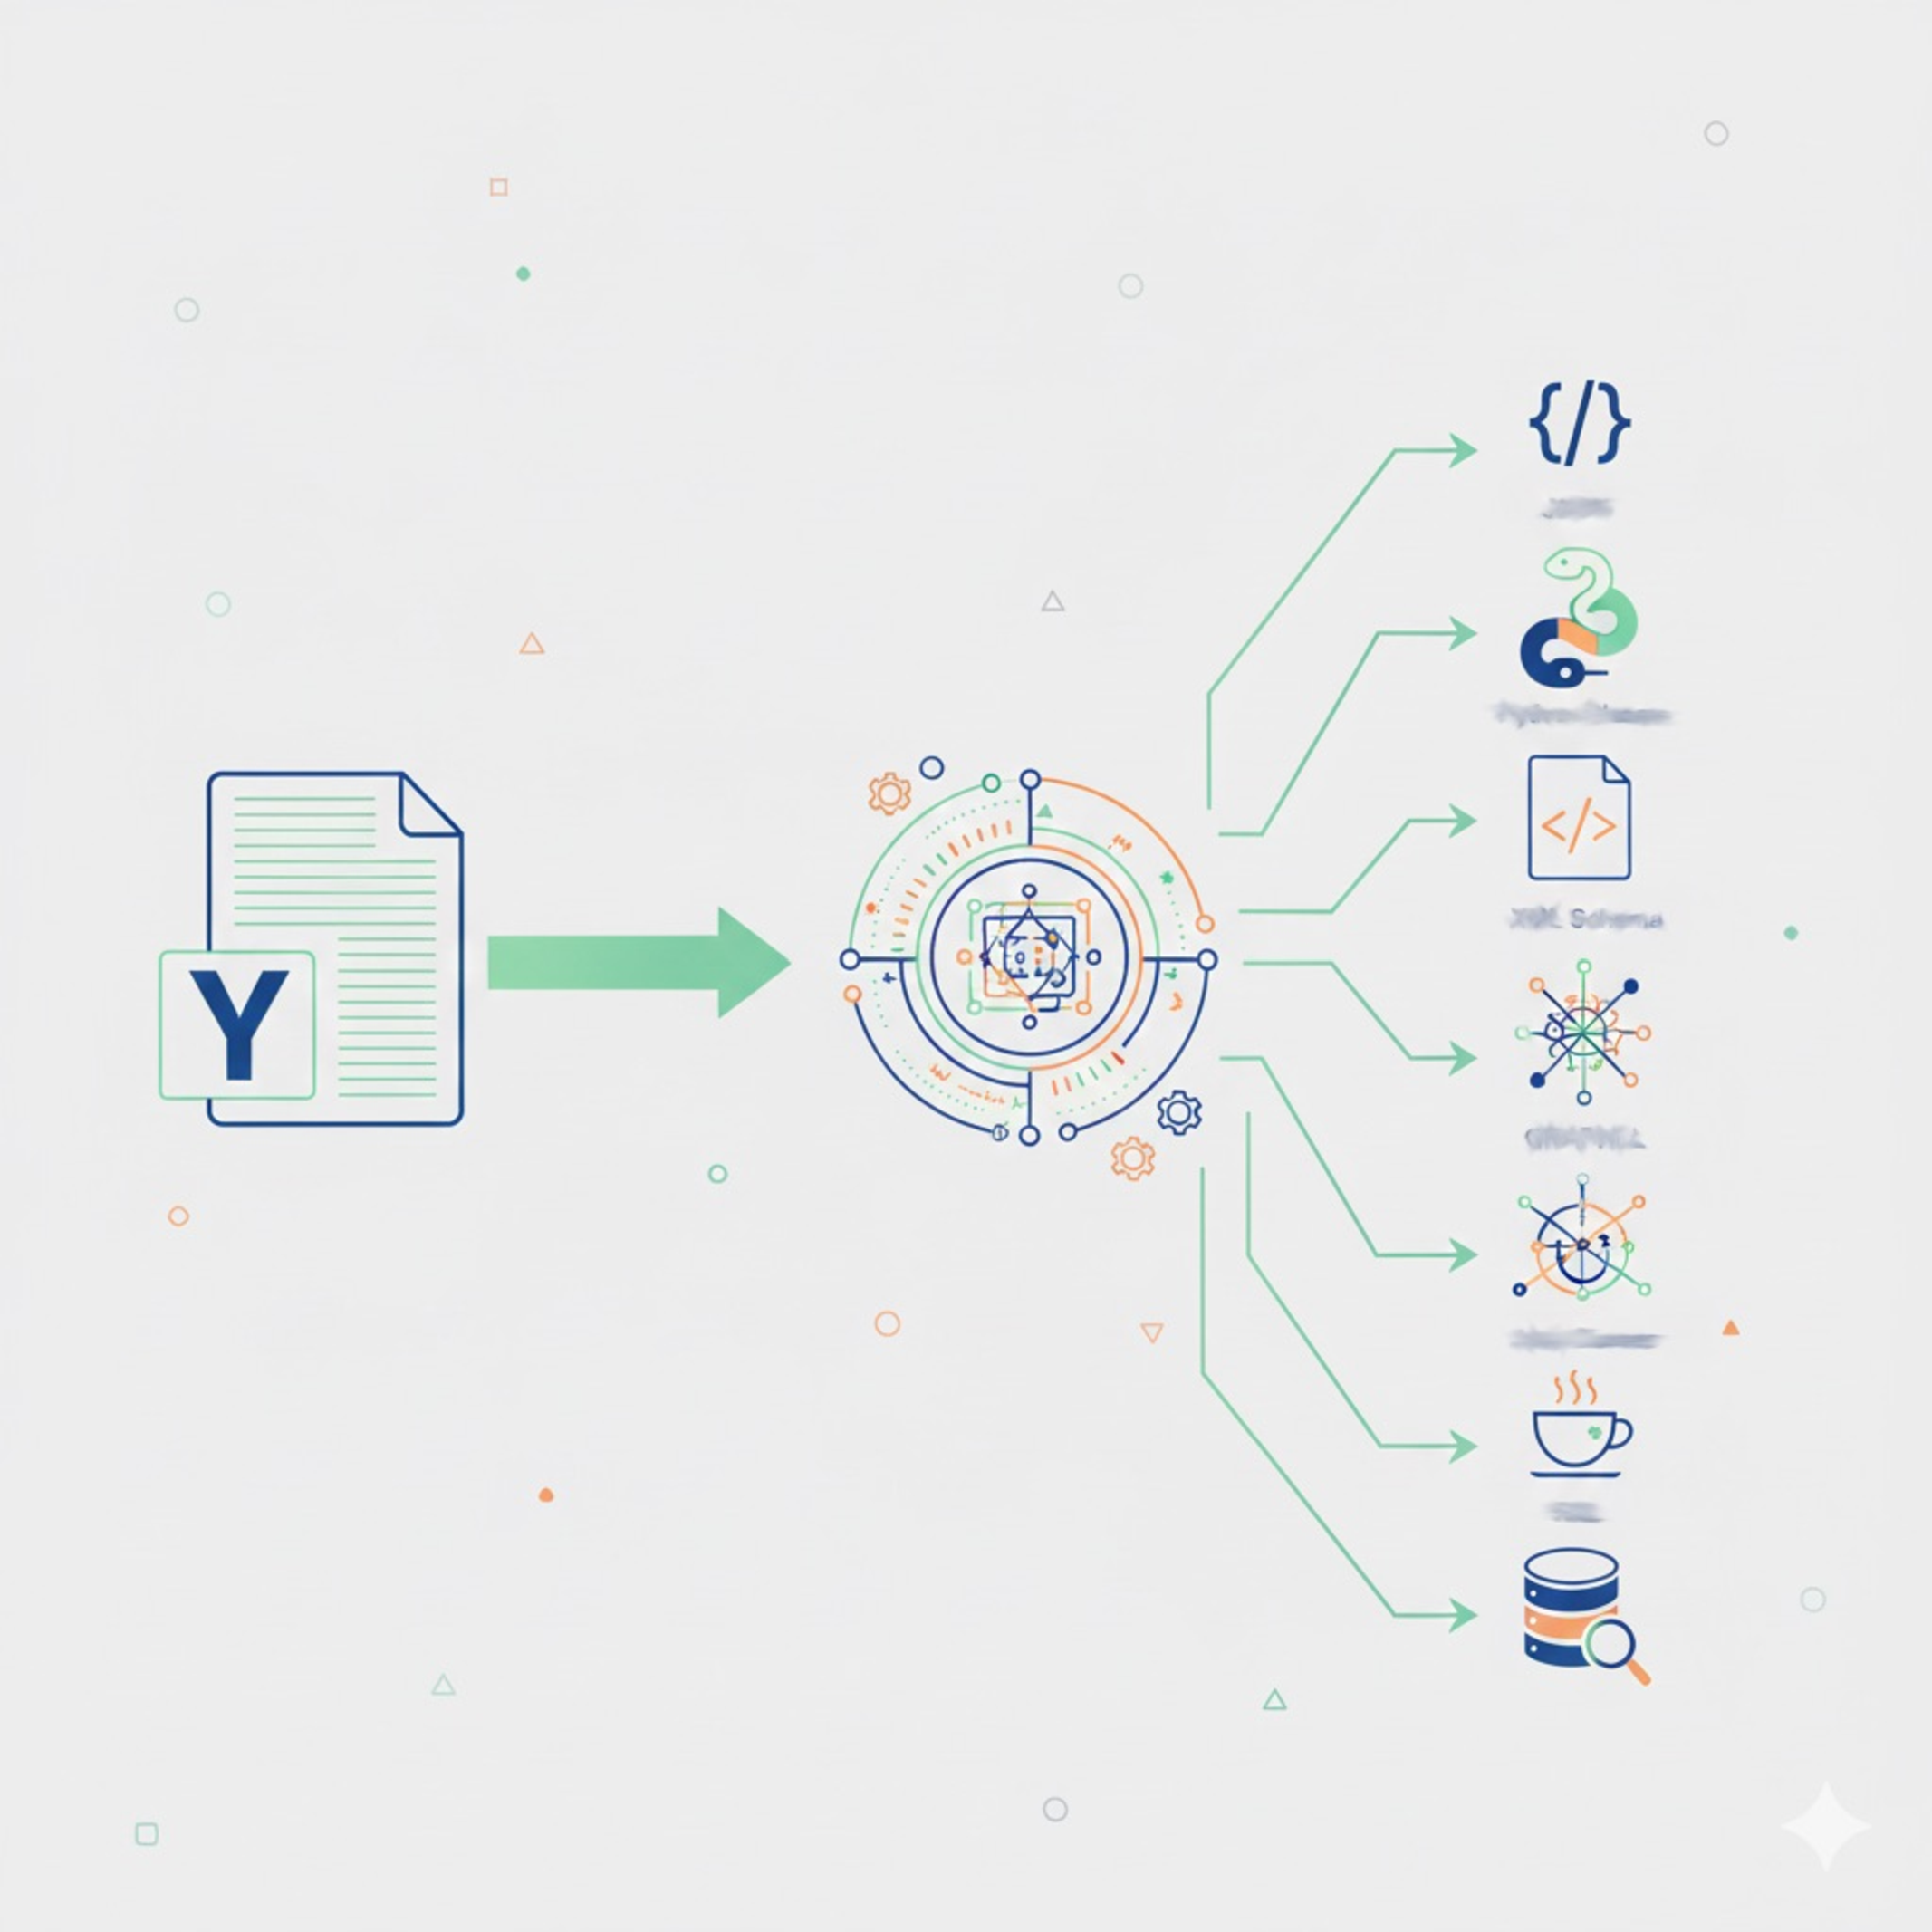
\includegraphics[width=0.8\textwidth]{figs/fig_d2p5/fig_d2p5_02-lnkml}
            \captionof{figure}{One Model $\rightarrow$ Many Formats}
        \end{center}
        \column{.64\textwidth}
        You write one simple `schema.yaml` file...
        \pause
        LinkML \textbf{auto-generates} all of these:
        \begin{itemize}
            \item \textbf{JSON-Schema} (for validation)
            \item \textbf{Python Classes} (for your scripts)
            \item \textbf{XML Schema (XSD)} (for your archive)
            \item \textbf{GraphQL} (for your web API)
        \end{itemize}
        \pause
        It is the \textbf{ultimate} tool for Interoperability ('I').
    \end{columns}
\end{frame}

\begin{frame}{Interactive: The Power of CVs and LinkML}{Module 5.2: Practice}
    \begin{block}{Discussion (10 min)}
        \textbf{Task:}
        \begin{itemize}
            \item \textbf{Explain} in your own words how a CV stops researchers from "making up" metadata terms.
            \pause
            \item \textbf{Explain} how LinkML solves the "XML vs. JSON" problem we had in Module 4. (Answer: It generates \textit{both} from one source!)
        \end{itemize}
        \pause
        \textbf{Goal:} \textbf{Explain} how these tools enable 'I'.
    \end{block}
\end{frame}

\begin{frame}{Learning Objectives (5.3)}
    \begin{itemize}
        \item \textbf{Map} free-text keywords to standardised terms in a \textit{domain-specific thesaurus}.
        \item \textbf{Map} classes and properties between two existing ontologies using \textbf{Protégé}.
    \end{itemize}
\end{frame}

\begin{frame}{Theory: Mapping Free-Text}{Module 5.3: Map}
    Mapping is the process of \emph{translating} your messy, free-text "internal" terms to the clean, public "standard" terms.
    
    \begin{block}{Example: Mapping to a Thesaurus}
        \begin{itemize}
            \item \textbf{Your Term:} "Pressure"
            \pause
            \item \textbf{Thesaurus:} `Gemet`
            \item \textbf{Search "Pressure":} Find `http://.../atmospheric\_pressure`
            \pause
            \item \textbf{Mapping:} Your `pressure` $\rightarrow$ `owl:equivalentClass` $\rightarrow$ `gemet:atmospheric\_pressure`
        \end{itemize}
    \end{block}
    You have now made your data interoperable with everyone else who uses the `Gemet` thesaurus.
\end{frame}

\begin{frame}{Theory: Mapping in Protégé}{Module 5.3: Map}
    Protégé is the tool for mapping two complex \emph{ontologies}.
    
    \textbf{Scenario:}
    \begin{itemize}
        \item `Ontology\_A` (from Biology) has a class: `Human`
        \item `Ontology\_B` (from Medicine) has a class: `Patient`
    \end{itemize}
    \pause
    Are these the same?
    \pause
    \begin{block}{Mapping Axioms in Protégé}
        \begin{itemize}
            \item `Ontology\_A:Human` $\rightarrow$ `owl:equivalentClass` $\rightarrow$ `Ontology\_B:Patient`
            (This means they are identical)
            \pause
            \item `Ontology\_A:Human` $\rightarrow$ `rdfs:subClassOf` $\rightarrow$ `Ontology\_B:Patient`
            (This means all Humans are Patients, but not all Patients are Humans - maybe some Patients are animals?)
        \end{itemize}
    \end{block}
    This logic is the core of semantic interoperability.
\end{frame}

\begin{frame}{Interactive: Mapping Workshop}{Module 5.3: Practice}
    \begin{block}{Workshop: Two Tracks (15 min)}
        \begin{columns}
            \column{.5\textwidth}
            \begin{block}{Track 1: Thesaurus}
                \textbf{Goal:} \textbf{Map} free-text.
                \pause
                \begin{itemize}
                    \item Go to a public thesaurus (e.g., `Gemet`, `AGROVOC`).
                    \item Find a term for "soil".
                    \item Find the URI.
                \end{itemize}
            \end{block}
            
            \column{.5\textwidth}
            \begin{block}{Track 2: Protégé (Demo)}
                \textbf{Goal:} \textbf{Map} two classes.
                \pause
                \begin{itemize}
                    \item (Live Demo)
                    \item Load two simple ontologies.
                    \item Create an `owl:equivalentClass` axiom between two classes.
                \end{itemize}
            \end{block}
        \end{columns}
    \end{block}
\end{frame}

\begin{frame}{Learning Objectives (5.4)}
    \begin{itemize}
        \item \textbf{Assess} a metadata record to \textbf{identify} free-text entries that should be replaced by a CV.
        \item \textbf{Assess} a candidate \textbf{LinkML schema} to \textbf{identify} structural conflicts.
    \end{itemize}
\end{frame}

\begin{frame}[fragile]{Theory: Assessing a Metadata Record}{Module 5.4: Assess}
\begin{columns}
    \column{.5\textwidth}
    \begin{block}{A "Bad" Metadata Record (Free-Text)}
\begin{lstlisting}[language=json]
{
  "title": "My Test",
  "material": "Steel",
  "measurement": "Toughness"
}
\end{lstlisting}
    \end{block}
        
    \column{.5\textwidth}
    \begin{block}{An "Assessed \& Improved" Record (CV)}
\begin{lstlisting}[language=json]
{
  "title": "My Test",
  "material": "emmo:SS-304",
  "measurement": "omat:Charpy_Impact_Test"
}
\end{lstlisting}
    \end{block}
\end{columns}
    \pause
    \textbf{Assessment:}
    \begin{itemize}
        \item What is "Steel"? (Which grade? `SS-304`? `SS-316`?)
        \item What is "Toughness"? (Charpy test? Izod test?)
    \end{itemize}
    \pause

    We \textbf{identified} the free-text and \textbf{replaced} it with URIs from a CV.
\end{frame}

\begin{frame}[fragile]{Theory: Assessing a LinkML Schema}{Module 5.4: Assess}

    \textbf{Problem:} You try to merge two data models (schemas) using LinkML.
    \bigskip
    
    \begin{columns}
        \column{.36\textwidth} 
        \begin{block}{Model A}
            \begin{lstlisting}[language=yaml]
classes:
  Sample:
    slots:
      ID:
        identifier: true
            \end{lstlisting}
        \end{block}
        \pause
        \column{.36\textwidth}
        \begin{block}{Model B}
            \begin{lstlisting}[language=yaml]
classes:
  Specimen:
    slots:
      UUID:
        identifier: true
            \end{lstlisting}
        \end{block}
        
    \end{columns}
    \vfill
    \pause
    \textbf{Assessment:} You have a \textbf{structural conflict}. `Sample` and `Specimen` are probably the same thing (`owl:equivalentClass`), but they have different identifier names (`ID` vs. `UUID`). LinkML helps you \textbf{identify} and \textbf{map} these conflicts.
\end{frame}

\begin{frame}[fragile]{Interactive: Find the Free-Text}{Module 5.4: Practice}
    \begin{block}{Activity (10 min)}
        \textbf{Task:} Look at this "bad" metadata record. \textbf{Assess} it and \textbf{identify} all the ambiguous free-text fields that need to be replaced by a CV.
\begin{lstlisting}[language=json]
{
  "author": "M. Schmidt",
  "date": "Oct 10, 2024",
  "location": "CN, Bldg 301",
  "instrument": "Zeiss Scope",
  "material": "Copper",
  "result": "Good"
}
\end{lstlisting}
        \pause
        \textbf{Answers:} `author` (needs ORCID), `date` (needs ISO format), `location` (needs URI), `instrument` (needs ID), `material` (needs URI), `result` (needs vocab).
    \end{block}
\end{frame}

\begin{frame}{Learning Objectives (5.5)}
    \begin{itemize}
        \item \textbf{Justify} the selection of a specific \textbf{ontology} over a simpler \textbf{controlled vocabulary}.
        \item \textbf{Justify} the decision to use an advanced feature in \textbf{Protégé} (e.g., reasoners).
    \end{itemize}
\end{frame}
\begin{frame}{Theory: CV vs. Ontology}
    \frametitle{Module 5.5: Justify}
    When do you need the complexity of an ontology?
    
    \begin{columns}
        \column{.5\textwidth}
        \begin{block}{Use a Controlled Vocabulary (CV)}
            \textbf{When:} You need to \emph{standardise input}.
            \begin{itemize}
                \item Drop-down lists.
                \item Simple tags.
                \item Harmonising keywords.
            \end{itemize}
            \textbf{Query:} "Find all data tagged with `Karlsruhe`."
        \end{block}
        
        \column{.5\textwidth}
        \begin{block}{Use an Ontology}
            \textbf{When:} You need to ask \emph{complex, logical questions}.
            \begin{itemize}
                \item `Experiment` \emph{uses\_material} `Steel`
                \item `Steel` \emph{has\_component} `Iron`
            \end{itemize}
            \textbf{Query:} "Find all experiments that used a material which has Iron as a component."
        \end{block}
    \end{columns}
    \pause
    \textbf{Justification:} You \textit{must} use an ontology if your research questions require logical inference.
\end{frame}

\begin{frame}{Theory: Protégé Reasoners}{Module 5.5: Justify}
    \begin{columns}
        \column{.36\textwidth}
        \begin{center}
            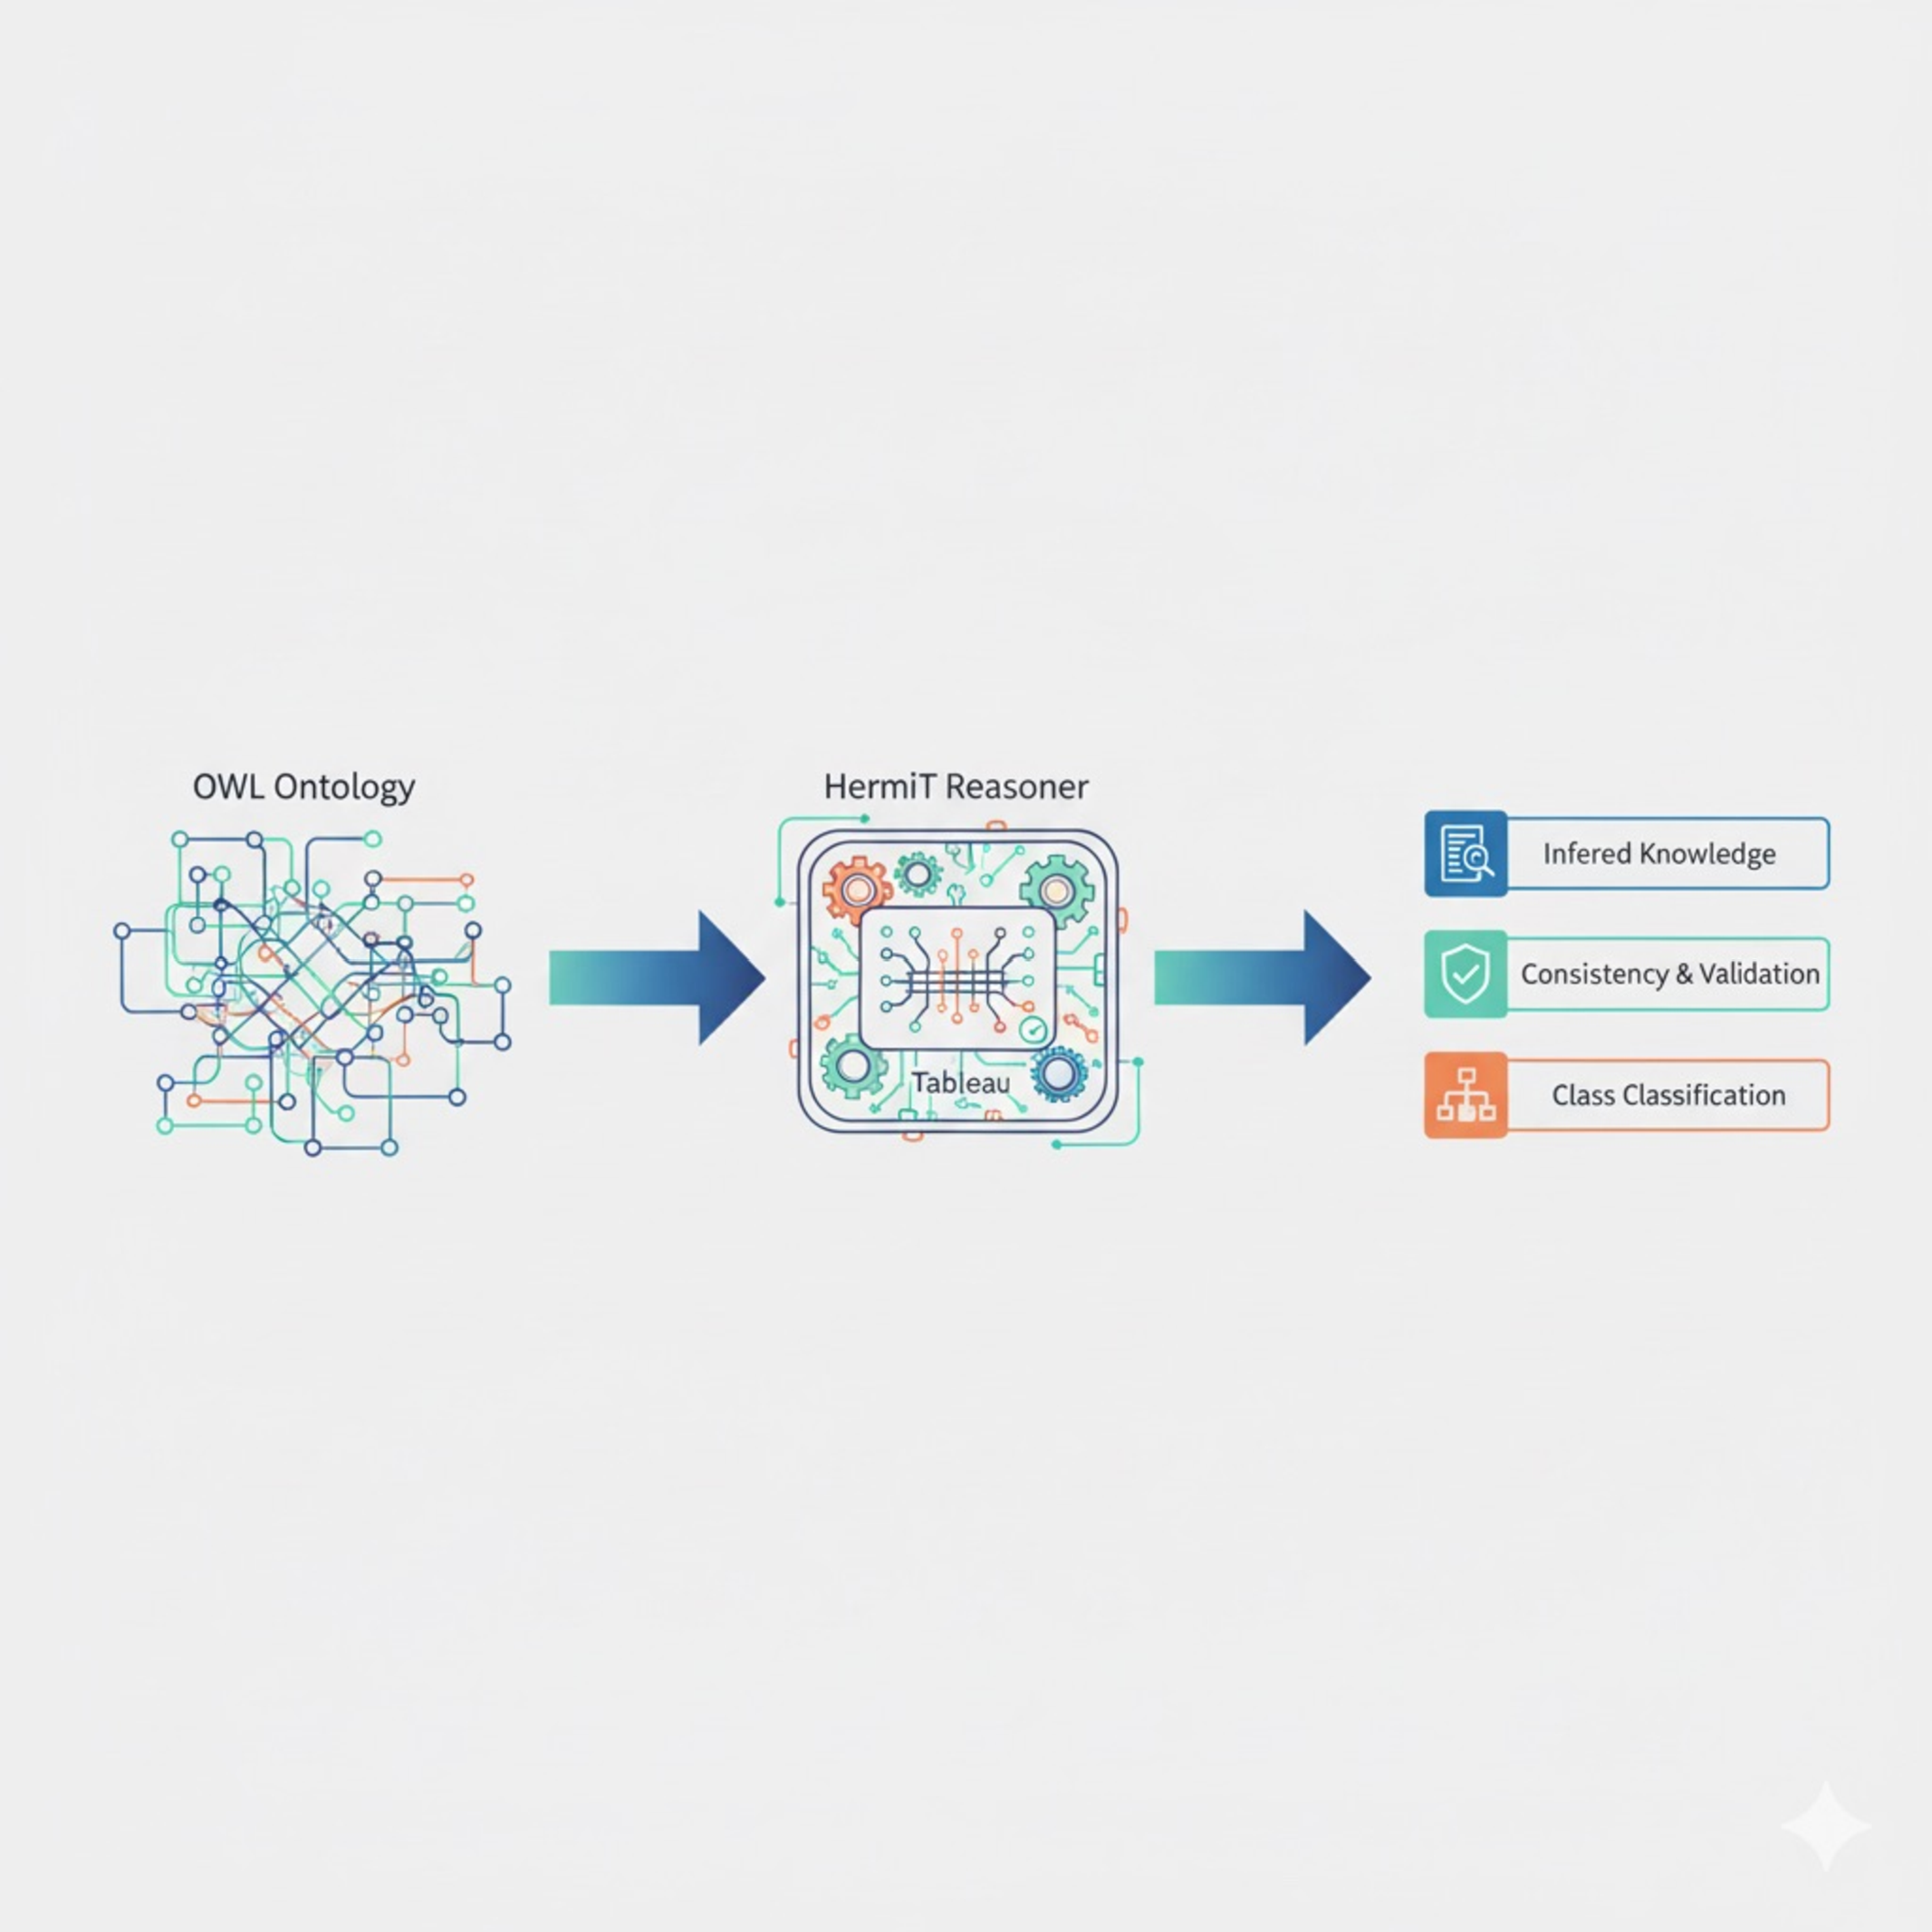
\includegraphics[width=0.8\textwidth]{figs/fig_d2p5/fig_d2p5_03-hermit}
            \captionof{figure}{A reasoner is a "logic engine" for your ontology.}
        \end{center}
        \column{.74\textwidth}
        You state the facts. The reasoner finds the hidden knowledge.
        \pause
        \begin{itemize}
            \item \textbf{You state:} `Karlsruhe` \emph{is\_a} `City`.
            \item \textbf{You state:} `City` \emph{is\_a} `Populated\_Place`.
            \pause
            \item \textbf{Reasoner infers:} `Karlsruhe` \emph{is\_a} `Populated\_Place`. (Transitivity)
        \end{itemize}
        \pause
        \textbf{Justification:} You \textit{must} use a reasoner to \textbf{validate the semantic consistency} of your model. If you state `A` is a `B`, and `B` is a `C`, but also `A` \emph{cannot} be a `C` (disjoint), the reasoner will raise an error and tell you your logic is broken.
            
    \end{columns}
\end{frame}

\begin{frame}{Interactive: Vocab or Ontology?}{Module 5.5: Practice}
    \begin{block}{Scenario (15 min)}
        \textbf{Task:} For each scenario, \textbf{justify} your choice: a simple \textbf{CV} or a full \textbf{Ontology}?
        \pause
        \begin{itemize}
            \item \textbf{Scenario 1:} You want to standardise the "Country" field in a user sign-up form.
            \item \emph{Answer:} \textbf{CV}. (A simple list).
            \pause
            \item \textbf{Scenario 2:} You want to model the entire energy grid, including power plants, substations, and the flow of electricity between them, to find weak points.
            \item \emph{Answer:} \textbf{Ontology}. (Needs complex relationships).
            \pause
            \item \textbf{Scenario 3:} You want to validate that your semantic mappings between two models are logical and not contradictory.
            \item \emph{Answer:} \textbf{Ontology with a Reasoner}.
        \end{itemize}
    \end{block}
\end{frame}
\begin{frame}{Learning Objectives (5.6)}
    \begin{itemize}
        \item \textbf{Develop} a simple, internal \textbf{controlled vocabulary} (CV) for an ELN template.
        \item \textbf{Develop} a \textbf{LinkML data model} that expresses semantic similarities identified via mapping.
    \end{itemize}
\end{frame}

\begin{frame}{Interactive: Draft an Internal CV}{Module 5.6: Practice}
    \begin{block}{Activity (10 min)}
        \textbf{Task:} Let's \textbf{develop} a simple internal CV for our ELN.
        \pause
        \textbf{Field:} `experiment\_status`
        \pause
        \textbf{Brainstorm:} What are the allowed terms?
        \begin{itemize}
            \item `planning`
            \item `active`
            \item `paused`
            \item `completed`
            \item `failed`
        \end{itemize}
        \pause
        \textbf{Result:} You have just created a CV! You can now build this into your ELN as a drop-down list to prevent "free-text" like "done" or "finished".
    \end{block}
\end{frame}

\begin{frame}[fragile]{Interactive: Draft a LinkML Model}{Module 5.6: Practice}
    \begin{block}{Challenge: Draft a LinkML Model (15 min)}
        \textbf{Task:} Remember our mapping: `Model A: Sample` and `Model B: Specimen`. \\
        \pause
        \textbf{Goal:} \textbf{Develop} a LinkML model that merges them. \\
        \pause
        \textbf{Solution (YAML):}
        \begin{columns}
            \column{.36\textwidth}
\begin{lstlisting}[language=yaml]
classes:
  MyMergedClass:
    # We map to BOTH ontologies
    is_a: ModelA:Sample
    exact_mappings:
      - ModelB:Specimen
    slots:
      # We merge the slots
      - ID
      - UUID
\end{lstlisting}

        \end{columns}
        \pause
        This LinkML model now formally expresses the semantic similarity.
    \end{block}
\end{frame}

\begin{frame}{Module 5: Summary}
    \begin{itemize}
        \item \textbf{Semantics} ('I') is about shared \emph{meaning}, not just format.
        \item We use a "ladder" of tools: \textbf{CVs} (lists), \textbf{Thesauri} (hierarchy), \textbf{Ontologies} (logic).
        \item \textbf{Protégé} is the tool for building and mapping ontologies.
        \item \textbf{LinkML} is the tool for building and merging data models.
        \item We must \textbf{map} our free-text to standard terms.
    \end{itemize}
    \vfill
    \begin{center}
        \textbf{End of Part 5}
    \end{center}
\end{frame}

% ===================================================================
% PART 6: Publish Metadata
% ===================================================================

\section{Publishing: KITOpen and OEP}

\begin{frame}{Day 2 - Part 6: Publishing Your Metadata}{12:15 - 13:00}
    \begin{block}{Module 6 Goal}
        The final step! Making your data public, findable, and accessible using our key platforms: \textbf{KITOpen} and the \textbf{Open Energy Platform (OEP)}.
    \end{block}
    \begin{center}
        
\includegraphics[width=0.36\textwidth]{figs/fig_d2p6/fig_d2p6_01-public}
        \captionof{figure}{From your lab (private) to the world (public).}
    \end{center}
\end{frame}

\begin{frame}{Learning Objectives (6.1)}
    \begin{itemize}
        \item \textbf{Identify} the mandatory submission fields for \textbf{KITOpen}.
        \item \textbf{List} the specific \textbf{domain-relevant metadata properties} unique to the \textbf{Open Energy Platform (OEP)}.
    \end{itemize}
\end{frame}

\begin{frame}{Theory: Institutional vs. Domain Repositories}{Module 6.1: Identify/List}
    \begin{columns}
        \column{.5\textwidth}
        \begin{block}{KITOpen (Institutional)}
            \textbf{Role:} Archives \emph{all} research output from KIT (papers, data, theses). \\
            \pause
            \textbf{Metadata:} General-purpose (Dublin Core). \\
            \pause
            \textbf{Mandatory Fields:}
            \begin{itemize}
                \item Title
                \item Creator (with KIT affiliation)
                \item Publication Year
                \item Resource Type (e.g., "Dataset")
                \item License
            \end{itemize}
        \end{block}
        
        \column{.5\textwidth}
        \begin{block}{Open Energy Platform (Domain)}
            \textbf{Role:} Archives \emph{only} energy research data, from \emph{all} institutions. \\
            \pause
            \textbf{Metadata:} Domain-specific. \\
            \pause
            \textbf{Domain-Relevant Properties:}
            \begin{itemize}
                \item `energy\_carrier\_type`
                \item `technology\_type`
                \item `geographic\_region (NUTS-3)`
                \item `temporal\_resolution`
            \end{itemize}
            \vspace{3.2ex}
        \end{block}
    \end{columns}
\end{frame}

\begin{frame}{Interactive: Repository Scavenger Hunt}{Module 6.1: Practice}
    \begin{block}{Activity (10 min)}
        \textbf{Task:} Open the websites for `KITOpen` and `OEP`.
        \pause
        \begin{itemize}
            \item Find the "Upload" or "Submit" page for new data.
            \item \textbf{Identify} 3 mandatory fields in KITOpen.
            \item \textbf{List} 3 \emph{domain-specific} fields in OEP that KITOpen does not have.
        \end{itemize}
        \pause
        \textbf{Discussion:} Why does OEP ask for `temporal\_resolution` while KITOpen doesn't?
    \end{block}
\end{frame}

\begin{frame}{Learning Objectives (6.2)}
    \begin{itemize}
        \item \textbf{Summarise} the process by which \textbf{KITOpen} assigns a PID (DOI) and fulfils 'F'.
        \item \textbf{Illustrate} how the community standards enforced by \textbf{OEP} enhance 'I'.
    \end{itemize}
\end{frame}

\begin{frame}{Theory: KITOpen and 'Findable'}{Module 6.2: Summarise}
    
    \begin{columns}
        \column{.36\textwidth} 
        \begin{center}
            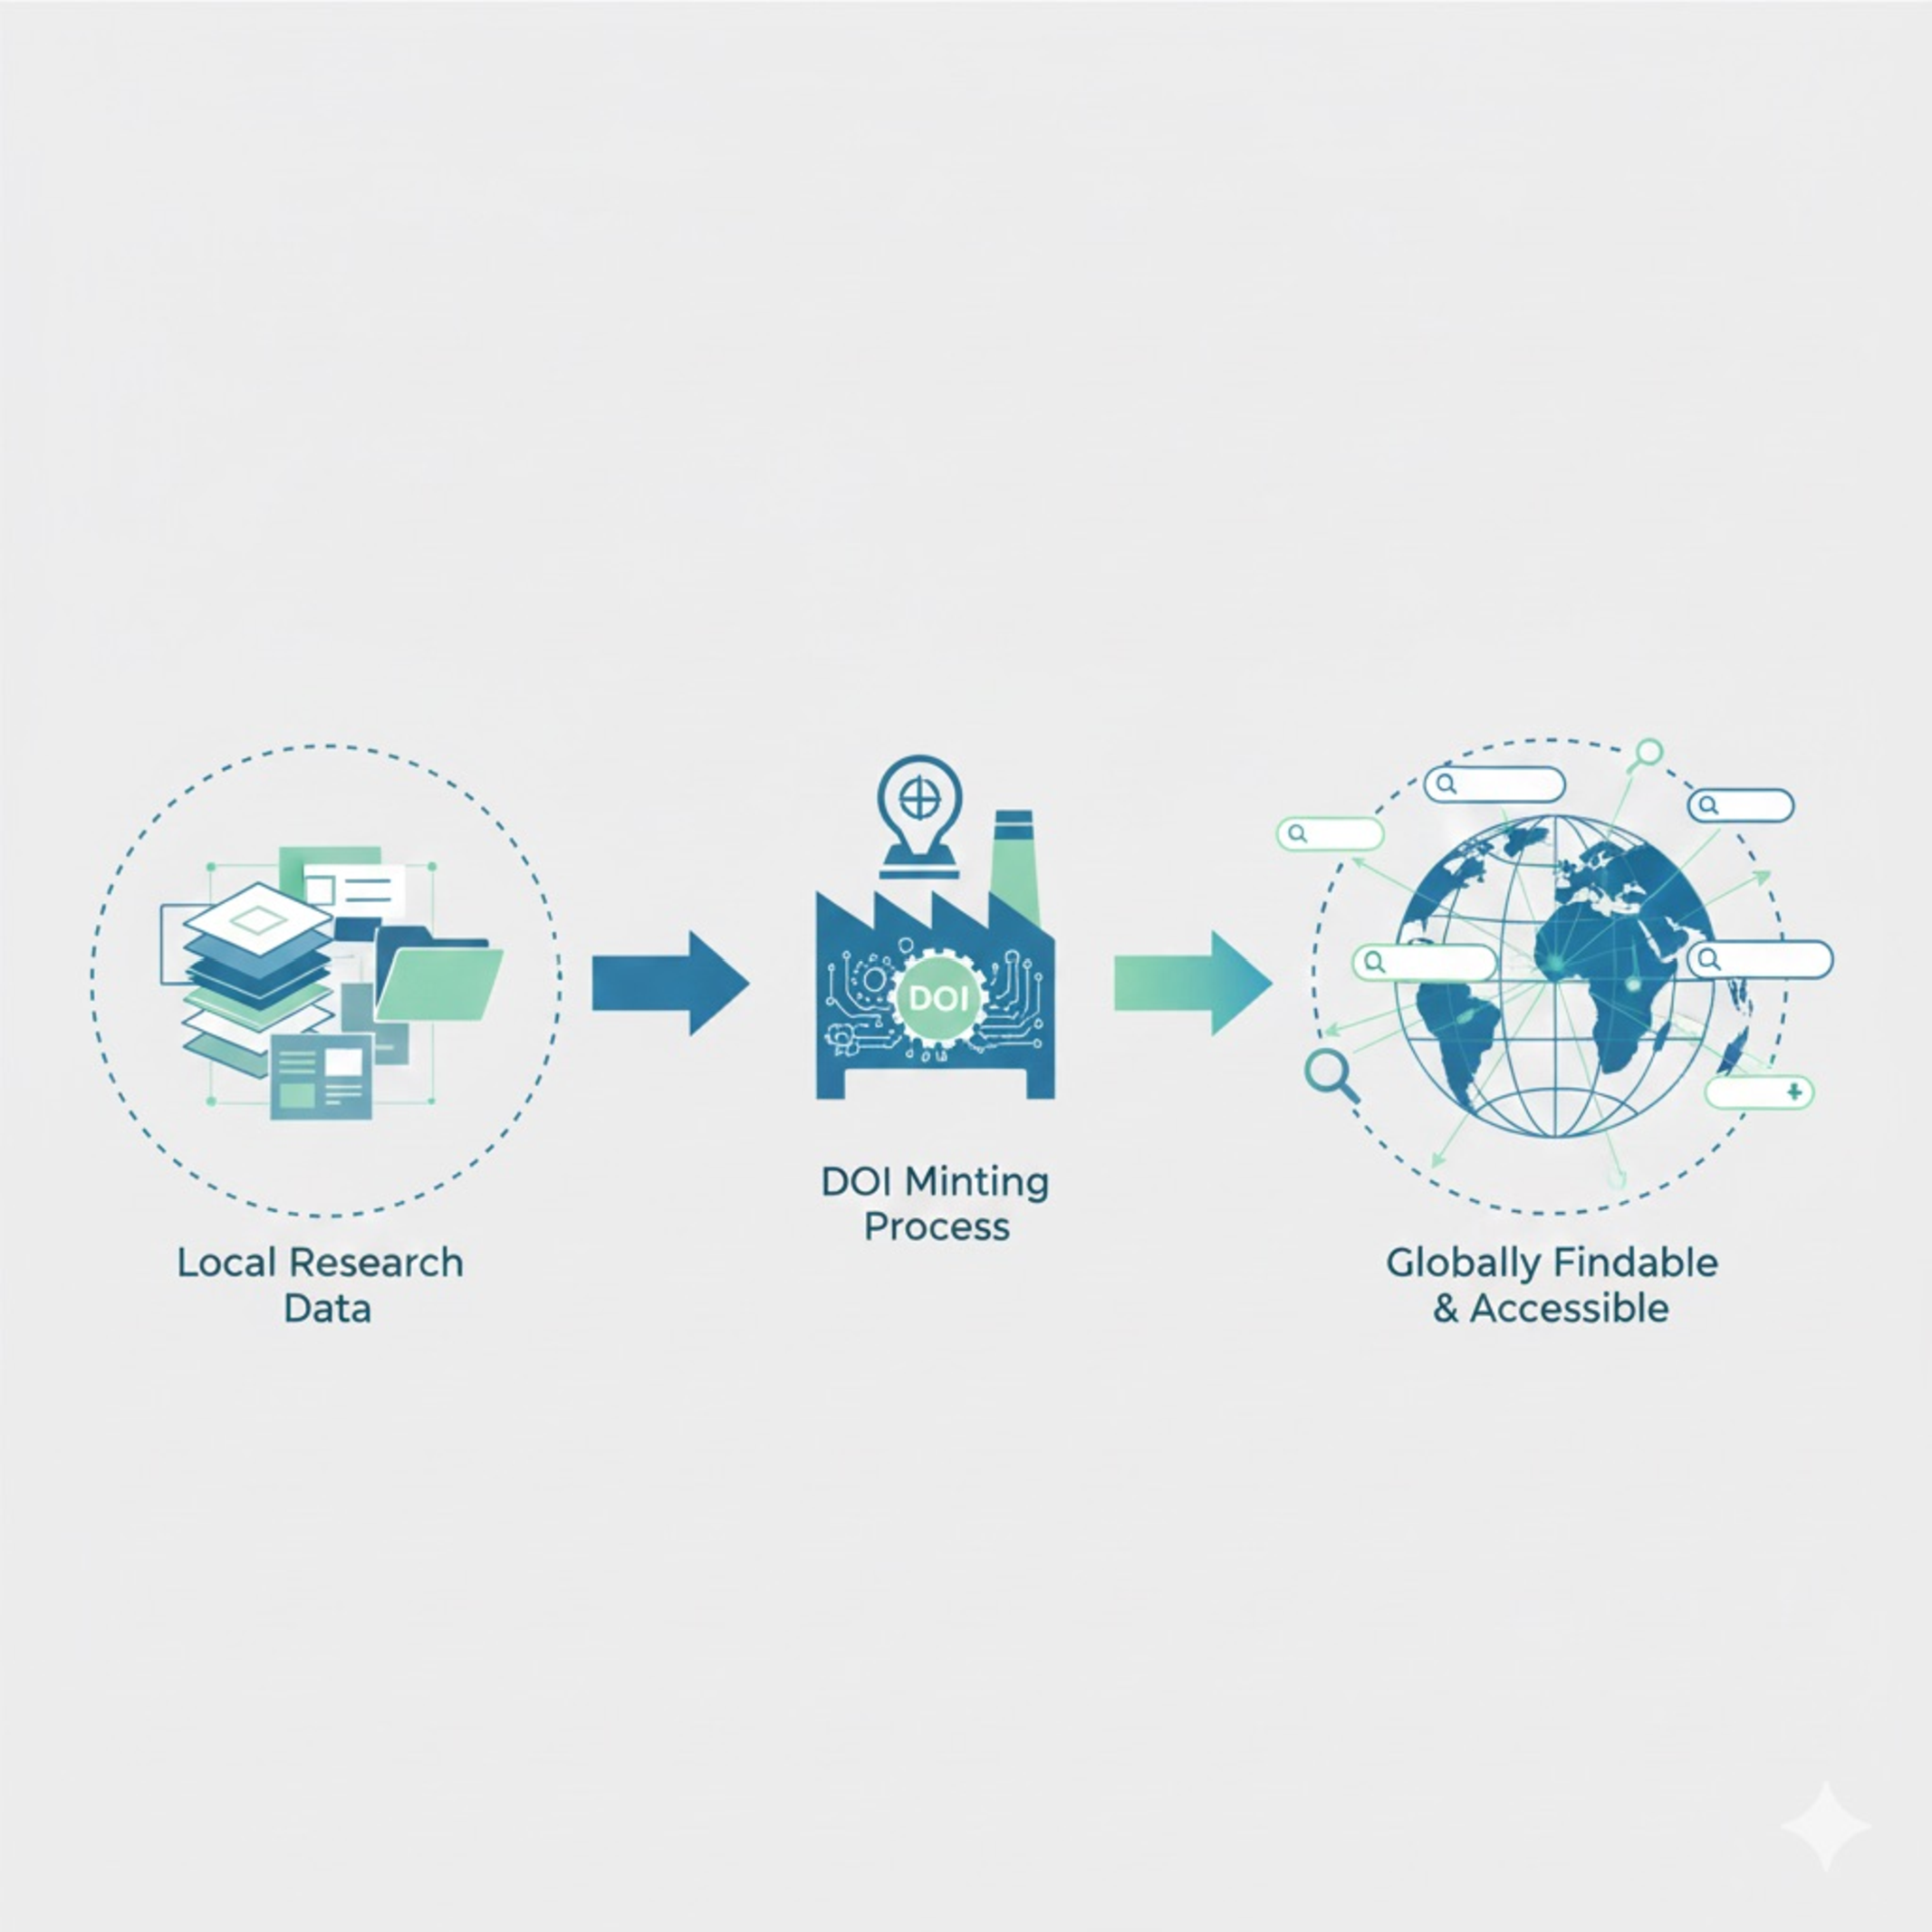
\includegraphics[width=.8\textwidth]{figs/fig_d2p6/fig_d2p6_02-mint}
            \captionof{figure}{The DOI Minting Process}
        \end{center}
        \column{.74\textwidth}
        \begin{enumerate}
            \item You upload your data to KITOpen.
            \pause
            \item You fill in the metadata (Title, Creator, etc.).
            \pause
            \item You click "Publish."
            \pause
            \item KITOpen (as a DataCite member) sends your metadata to the DOI registration agency.
            \pause
            \item A new, unique \textbf{DOI} (e.g., `10.5445/IR/100...`) is created and permanently linked to your data's metadata page on KITOpen.
        \end{enumerate}
    \end{columns}

    \pause
    Your data is now globally \textbf{Findable}.
\end{frame}

\begin{frame}{Theory: OEP and 'Interoperable'}{Module 6.2: Illustrate}
    The OEP's community standards (its metadata schema) are its power.
    
    \begin{block}{How OEP Enhances 'I'}
        \textbf{Problem:}
        \begin{itemize}
            \item You have a dataset of German power grids.
            \item A researcher from France has a dataset of French power grids.
        \end{itemize}
        \pause
        \textbf{Solution:}
        \begin{itemize}
            \item The OEP \emph{forces} both of you to use the \emph{same metadata fields} (e.g., `energy\_carrier\_type`) and the \emph{same vocabularies}.
            \pause
            \item \textbf{Result:} A third person can now write \emph{one script} to query and automatically combine both your dataset and the French dataset.
        \end{itemize}
    \end{block}
    This is \textbf{Interoperability} in action, enforced by a domain repository.
\end{frame}

\begin{frame}{Interactive: The Role of Each Repo}{Module 6.2: Practice}
    \begin{block}{Discussion (10 min)}
        \textbf{Task:}
        \begin{itemize}
            \item \textbf{Summarise:} Why is getting a DOI from KITOpen better than just putting data on your lab website?
            \pause
            \item \textbf{Illustrate:} Draw a simple diagram showing how the OEP's common standard allows two different datasets (A and B) to be combined by a third party (C).
        \end{itemize}
    \end{block}
\end{frame}

\begin{frame}{Learning Objectives (6.3)}
    \begin{itemize}
        \item \textbf{Upload} a dataset and metadata file to \textbf{KITOpen}.
        \item \textbf{Populate} an \textbf{OEP} metadata template using controlled vocabularies.
    \end{itemize}
\end{frame}

\begin{frame}{Interactive: Mock Submission (KITOpen)}{Module 6.3: Practice}
    \begin{block}{Workshop (10 min)}
        \textbf{Task:} (Conceptual or Live Demo)
        \pause
        \begin{enumerate}
            \item Take the `metadata.json` file you created in Module 4.
            \pause
            \item Go to the KITOpen submission form.
            \pause
            \item \textbf{Upload} your (dummy) data file.
            \pause
            \item Manually copy the fields (Title, Creator, etc.) from your JSON file into the corresponding fields in the KITOpen web form.
        \end{enumerate}
        \pause
        \textbf{Goal:} \textbf{Upload} (conceptually) a dataset and populate the metadata.
    \end{block}
\end{frame}

\begin{frame}{Interactive: Mock Submission (OEP)}{Module 6.3: Practice}
    \begin{block}{Workshop (10 min)}
        \textbf{Task:} Go to the OEP submission template.
        \pause
        \textbf{Challenge:} Find the field for "Geographic Region."
        \pause
        \begin{itemize}
            \item It likely requires a \textbf{controlled vocabulary} (e.g., NUTS codes).
            \item You can't just type "Karlsruhe."
            \item \textbf{Find the NUTS code for Karlsruhe.} (It's `DE122`).
        \end{itemize}
        \pause
        \textbf{Goal:} \textbf{Populate} an OEP template using a required CV.
    \end{block}
\end{frame}

\begin{frame}{Learning Objectives (6.4)}
    \begin{itemize}
        \item \textbf{Differentiate} between the institutional schema (KITOpen) and a general schema (Dublin Core).
        \item \textbf{Compare} the required access policy settings between KITOpen and OEP.
    \end{itemize}
\end{frame}

\begin{frame}{Theory: Schema Mapping (DC vs. KITOpen)}{Module 6.4: Differentiate}
    \begin{itemize}
        \item \textbf{Dublin Core (DC):} Is general. It has 15 fields.
        \pause
        \item \textbf{KITOpen Schema:} Is specific. It \textit{includes} all of Dublin Core (this is called "DC-compliance"), but adds \textbf{institutional} fields.
        \pause
        \item \textbf{Analysis:}
        \begin{itemize}
            \item `DC:Creator` $\rightarrow$ `KITOpen:Creator` (Direct map)
            \item `DC:Rights` $\rightarrow$ `KITOpen:License` (Direct map)
            \pause
            \item `KITOpen:KIT\_Affiliation` $\rightarrow$ \textbf{No equivalent in DC!}
            \item `KITOpen:Project\_ID (DFG)` $\rightarrow$ \textbf{No equivalent in DC!}
        \end{itemize}
    \end{itemize}
    \pause
    \begin{block}{Conclusion}
        KITOpen's schema is an \emph{extension} of Dublin Core, enriched with fields that matter to KIT and its funders.
    \end{block}
\end{frame}

\begin{frame}{Theory: Comparing Access Policies}{Module 6.4: Compare}
    \begin{columns}
        \column{.5\textwidth}
        \begin{block}{KITOpen Access Policy}
            \begin{itemize}
                \item \textbf{Focus:} Institutional mandate.
                \item \textbf{Default:} As open as possible, as closed as necessary.
                \item \textbf{Options:} Open, Embargoed, Restricted (to KIT), Closed.
                \item Very flexible to support all disciplines (from humanities to engineering).
            \end{itemize}
        \end{block}
        
        \column{.5\textwidth}
        \begin{block}{OEP Access Policy}
            \begin{itemize}
                \item \textbf{Focus:} Community building.
                \item \textbf{Default:} Open Access (CC-BY).
                \item \textbf{Culture:} Strong push for openness. Restricted data is rare.
                \item Less flexible, as it serves a community with a shared goal of open, interoperable data.
            \end{itemize}
        \end{block}
    \end{columns}
\end{frame}

\begin{frame}{Interactive: Institutional vs. Domain}{Module 6.4: Practice}
    \begin{block}{Debate (15 min)}
        \textbf{Scenario:} You only have time to publish your energy dataset in \emph{one} repository.
        \pause
        \begin{columns}
            \column{.5\textwidth}
            \textbf{Group 1: Argue for KITOpen}
            \begin{itemize}
                \item Fulfils KIT mandate
                \item Long-term preservation guarantee
                \item Flexible access
            \end{itemize}
            
            \column{.5\textwidth}
            \textbf{Group 2: Argue for OEP}
            \begin{itemize}
                \item Reaches your \textit{community}
                \item Higher impact in your field
                \item Better, richer metadata
            \end{itemize}
        \end{columns}
        \pause
        \textbf{Goal:} \textbf{Compare} policies and \textbf{Differentiate} schemas.
    \end{block}
\end{frame}

\begin{frame}{Learning Objectives (6.5)}
    \begin{itemize}
        \item \textbf{Appraise} a draft KITOpen record to ensure the selected \textbf{reuse license} (e.g., CC-BY) balances policy and FAIR principles.
        \item \textbf{Justify} the decision to \textbf{cross-reference} the OEP entry with a publication, assessing the benefit to \textbf{Findability}.
    \end{itemize}
\end{frame}

\begin{frame}{Theory: Appraising a License}{Module 6.5: Appraise}
When choosing a license on KITOpen, you must \textbf{appraise} the options.

\begin{columns}
    \column{.36\textwidth}
        \begin{center}
        
\includegraphics[width=0.72\textwidth]{figs/fig_d2p6/fig_d2p6_03-love.pdf}
    \end{center}

    \column{.74\textwidth}
    \begin{itemize}
        \item \textbf{CC0 / CC-BY:} \textbf{FAIR Principles}: Excellent! (Maximises 'R'eusable), \textbf{Institutional Policy:} Excellent! (Meets open access goals).
        \pause
        \item \textbf{CC-BY-NC-ND}: \textbf{FAIR Principles:} Poor! This license \emph{prevents} reusability ('R') by stopping others from combining your data or using it in new tools, \textbf{Institutional Policy:} Acceptable, but not preferred.
    \end{itemize}
    
\end{columns}
    \vspace{1.6ex}
    \pause
    \textbf{Appraisal:} Unless you have a strong legal/commercial reason, CC-BY is the best choice.
\end{frame}

\begin{frame}{Theory: The Power of Linking}{Module 6.5: Justify}
    
    \begin{columns}
        \column{.36\textwidth} 
        \begin{center}
            
\includegraphics[width=.8\textwidth]{figs/fig_d2p6/fig_d2p6_04-paths}
        \end{center}
        
        \column{.74\textwidth}
        \textbf{Justification:} Why link your OEP data to your journal paper?
        \pause
        
        \begin{itemize}
            \item \textbf{Path 1:} Researcher finds your \textbf{Paper}. The paper links to the \textbf{OEP} data (via DOI). $\rightarrow$ \textbf{Data is Found!}
            \pause
            \item \textbf{Path 2:} Researcher finds your \textbf{OEP Data}. The metadata links to the \textbf{Paper} (via DOI). $\rightarrow$ \textbf{Paper is Found!}
        \end{itemize}
        
        \pause
        
        By \textbf{cross-referencing}, you double the pathways to your work, dramatically increasing its \textbf{Findability} and potential \textbf{Impact}.
        
    \end{columns}
    
\end{frame}

\begin{frame}{Interactive: Appraise and Justify}{Module 6.5: Practice}
    \begin{block}{Discussion (10 min)}
        \textbf{Task 1: Appraise}
        \begin{itemize}
            \item Your colleague wants to use a `CC-BY-ND` (No-Derivatives) license "so nobody can misrepresent my data." \textbf{Appraise} this choice. Is it good for FAIR?
        \end{itemize}
        \pause
        \textbf{Task 2: Justify}
        \begin{itemize}
            \item \textbf{Justify} (in one sentence) why you must include your ORCID iD in your KITOpen submission. (Hint: It links your \textit{data} to your \textit{person}).
        \end{itemize}
    \end{block}
\end{frame}

\begin{frame}{Learning Objectives (6.6)}
    \begin{itemize}
        \item \textbf{Draft} the final, publicly visible \textbf{data citation} and \textbf{abstract} for a dataset, optimising for findability.
        \item \textbf{Synthesize} a final publication strategy that integrates \textbf{KITOpen} and \textbf{OEP}.
    \end{itemize}
\end{frame}

\begin{frame}{Theory: Writing a "Data Abstract"}{Module 6.6: Draft}
    Your Data Abstract is \textbf{not} your Paper Abstract. It's "SEO" for your data.
    
    \begin{columns}
        \column{.4\textwidth}
        \begin{block}{Bad Data Abstract}
            "This file contains the data for our recent paper. See the paper for details."
        \end{block}
        \vspace{3.2ex}
        \pause
        \textbf{Problem:} No keywords. No context. Not findable.
        
        \column{.6\textwidth}
        \begin{block}{Good Data Abstract}
            "This dataset contains raw data from a 2025 simulation of the German power grid, focusing on the NUTS-3 region of Karlsruhe (DE122). Data includes hourly load profiles and wind generation, modelled using [Software]... "
        \end{block}
        \pause
            \textbf{Result:} Rich with keywords. Highly findable.
    \end{columns}
\end{frame}

\begin{frame}{Theory: The "Both" Strategy}{Module 6.6: Synthesise}
    You don't have to choose between KITOpen and OEP. The best strategy is to use \textbf{both}.
    
    \begin{block}{The "HMC/KIT" Best Practice Strategy}
        \begin{enumerate}
            \item \textbf{Archive (Integrity):} Deposit the full, final, static dataset on \textbf{KITOpen}. This fulfils your institutional duty and gets a permanent DOI for long-term archiving.
            \pause
            \item \textbf{Index (Interoperability):} Create a \emph{new metadata record} on \textbf{OEP}.
            \pause
            \item \textbf{Link (Findability):} In the OEP record, do \textbf{not} re-upload the data. Instead, point to the \textbf{KITOpen DOI}.
        \end{enumerate}
    \end{block}
    \pause
    \textbf{Result:} You get the long-term integrity of KITOpen \emph{and} the domain-specific findability of OEP.
\end{frame}

\begin{frame}{Interactive: Your Final Strategy}{Module 6.6: Practice}
    \begin{block}{Final Activity (15 min)}
        \textbf{Task 1: Draft}
        \begin{itemize}
            \item Take 5 minutes and \textbf{draft} a "good" data abstract (2-3 sentences) for your own research data. Focus on keywords.
        \end{itemize}
        \pause
        \textbf{Task 2: Synthesise}
        \begin{itemize}
            \item \textbf{Synthesize} your final publication strategy. How will you use both your institutional and domain repositories?
            \item Share your plan.
        \end{itemize}
    \end{block}
\end{frame}

\begin{frame}{Workshop Summary}
    \begin{columns}
        \column{.5\textwidth}
        \begin{block}{Day 1: Foundations}
            \begin{itemize}
                \item Integrity $\rightarrow$ FAIR
                \item DMP $\rightarrow$ RDMO
                \item Operations $\rightarrow$ ELN, Git, Pipelines
            \end{itemize}
        \end{block}
        
        \column{.5\textwidth}
        \begin{block}{Day 2: Metadata}
            \begin{itemize}
                \item Serialisation (XML, JSON)
                \item Semantics (CV, Ontology)
                \item Publishing (KITOpen, OEP)
            \end{itemize}
        \end{block}
    \end{columns}
    \vfill
    \begin{block}{All Goals Achieved!}
        You can now connect Data Integrity to FAIR, build a DMP in RDMO, integrate RDM into operations, serialise and semantically enrich metadata, and publish on KITOpen and OEP.
    \end{block}
\end{frame}

\begin{frame}{Thank You}
    \begin{center}
        \vfill
        \Huge{\textbf{Questions?}}
        \vfill
        \vfill
        \large{Helmholtz Metadata Collaboration (HMC)} \\
        \large{Karlsruhe Institute of Technology (KIT)}
    \end{center}
\end{frame}

\end{document}